This chapter presents a framework for topology-editable surface
reconstruction from cross sections with arbitrary orientations, with
an emphasis on how the algorithm in Chapter~\ref{ch:orthsurf} is
generalized to handle cross sections with arbitrary orientations and
how the sketching technique is used in a topology editing process to
increase the flexibility of the reconstruction.

%%-----------------------------------------------------------------------------
\section{Introduction}
\label{ch6:sec:intro}

%introduction of surface reconstruction
In Chapter~\ref{ch:orthsurf} we have presented an algorithm on
surface  reconstruction from orthogonal cross sections, which
effectively supports the progressive modeling operation in our
sketching interface and avoids the limitations in the method
in~\cite{LBDLJ08}. However in some other applications such as the 3D
data recovery from medical data (CT, MRI, Ultrasound, etc.), terrain
modeling and so on, the input cross sections are usually lying on
planes with arbitrary orientations. In that case, the method in
Chapter~\ref{ch:orthsurf} cannot be directly used to solve this
problem. Though the work~\cite{LBDLJ08} proposed a general solution
to this problem, some challenges still exist and remain unsolved.

%challenges
First, the reconstructed surface, which usually represents a 3D
object, may contain multiple disconnected components (islands).
While in most cases, an object with just one single component is
often desired by the user. To avoid this problem we have proposed a strategy in Chapter~\ref{ch:orthsurf}, which is suitable for sketch-based modeling operations when the user iteratively adds new sketches close to the existing curves. However for the general-purpose surface reconstruction which reconstructs the surface from an existing set of cross sections, this problem still cannot be easily solved by using this strategy. What is worse, it may become more obvious for a large number of cross sections with arbitrary orientations and complex mutual relationship which may not occur in sketch-based modeling operations. In that case, it has been difficult to maintain both the interpolation on the input curves and regularity of the local shapes, letting alone the requirement of the single-component property.

Second, without the  prior information on the topology of the
target shape, the initial reconstruction result cannot be
guaranteed to completely meet the user's expectation. Once it is
not satisfactory, the user has to employ other editing tools to
further modify it to a desired shape, which is a totally
independent process of the reconstruction and may require laborious
work and complicated computation.

%anatomy example
\begin{figure*} [htbp]
  \centering
  \subfigure[]{
    \centering
     \begin{minipage}[b]{0.4\textwidth}
      \centering
      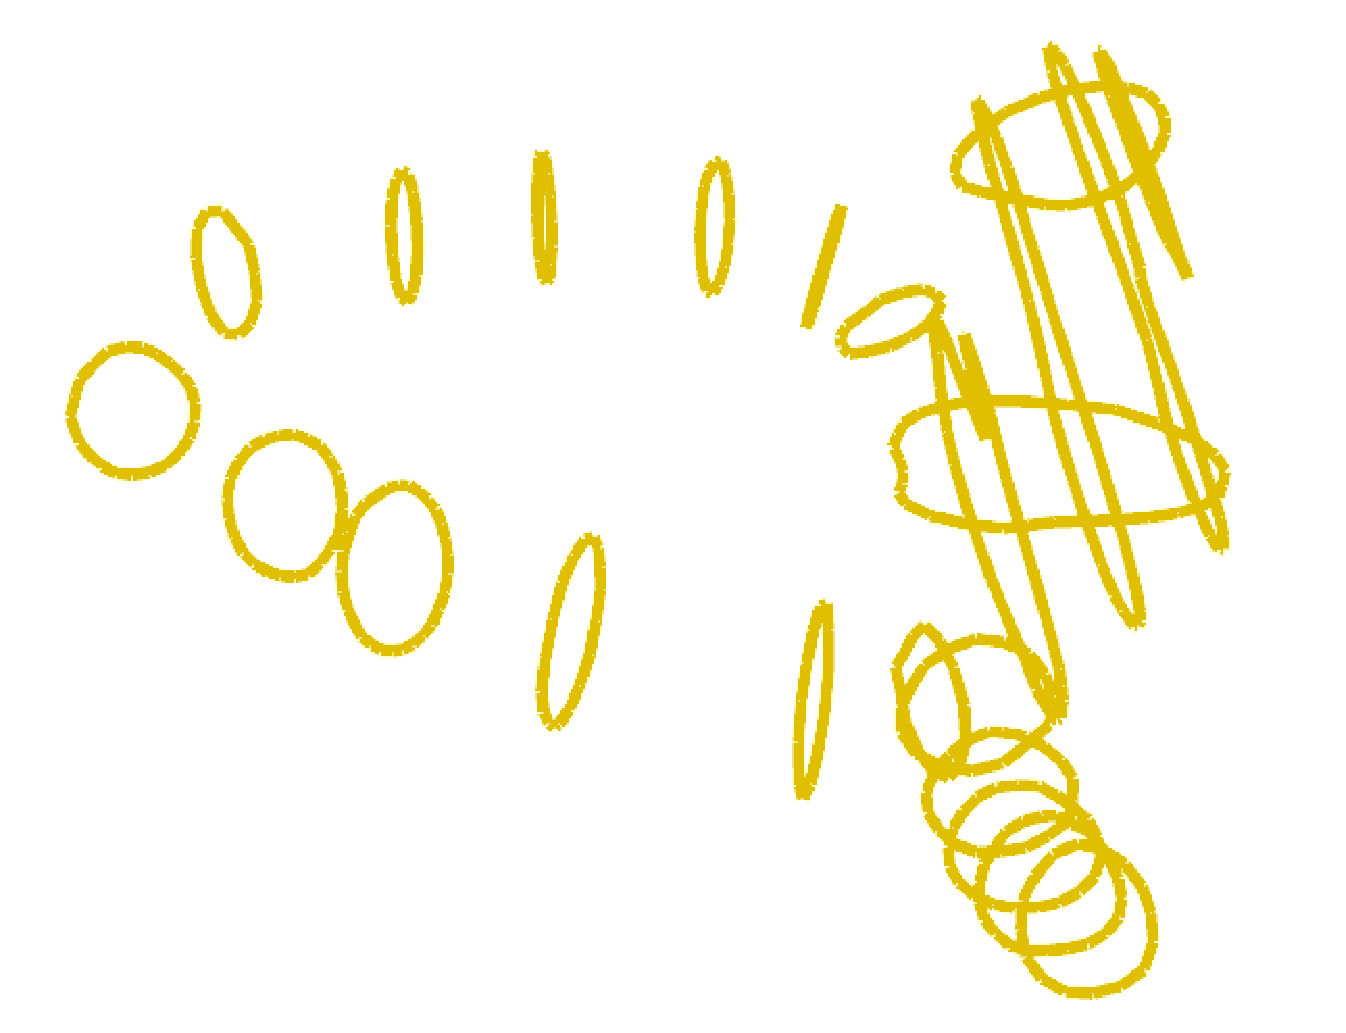
\includegraphics[scale=0.15]{figs/f6.anatomy-input.eps}%0.16
    \end{minipage}}
  \subfigure[]{
    \begin{minipage}[b]{0.4\textwidth}
      \centering
      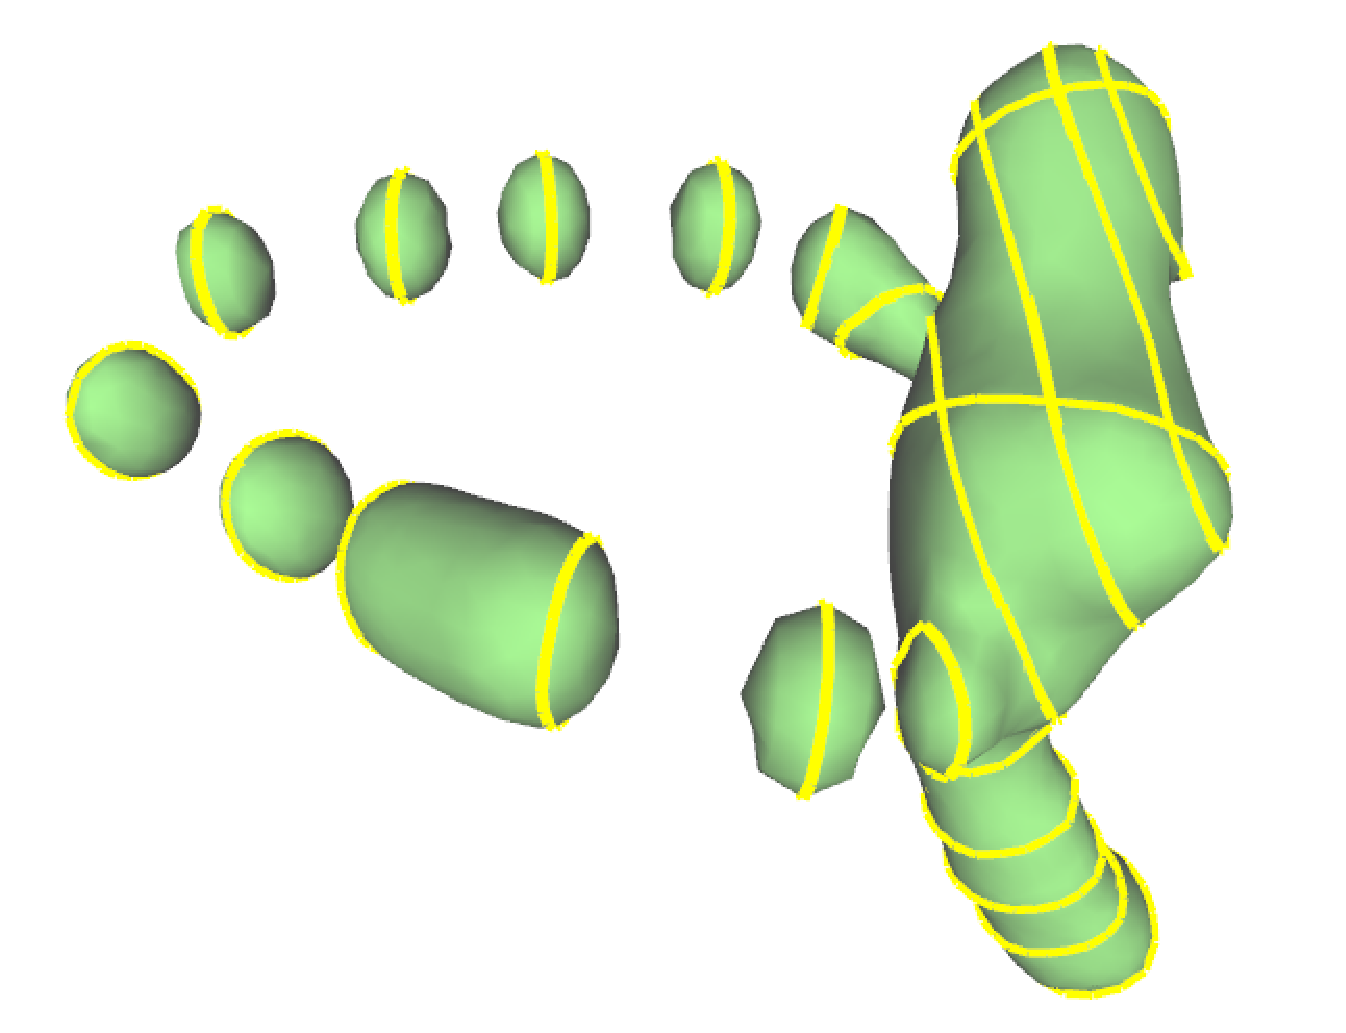
\includegraphics[scale=0.15]{figs/f6.anatomy-tj-result.eps}%0.16
    \end{minipage}}
  \caption{An example of surface reconstruction using Liu et al's
  algorithm \cite{LBDLJ08}.
  (a) Input cross sections.
  (b) The reconstructed result that has several disconnected components.}
  \label{fig:anatomy-ju}
\end{figure*}

\begin{figure*} [htbp]
  \centering
  \subfigure[]{
    \centering
    \label{fig:anatomy:b}
    \begin{minipage}[b]{0.23\textwidth}
      \centering
    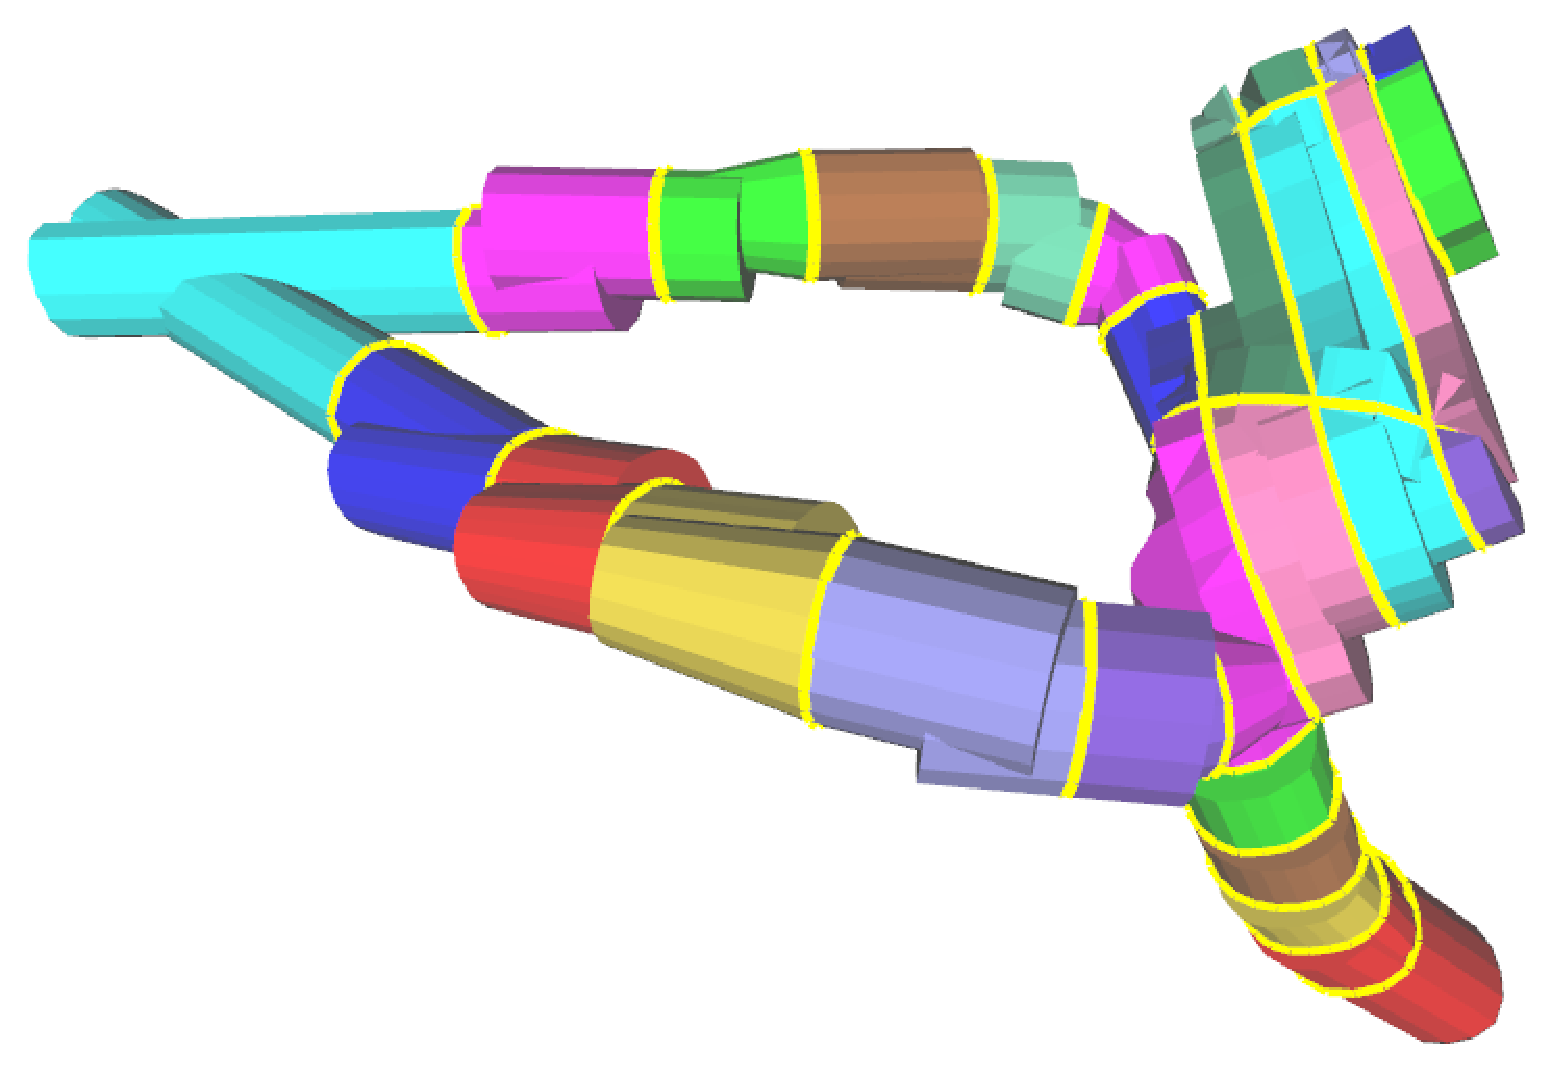
\includegraphics[scale=0.14]{figs/f6.anatomy-result-initial-union.eps}%0.15
    \end{minipage}}
  \subfigure[]{
    \centering
    \label{fig:anatomy:c}
    \begin{minipage}[b]{0.23\textwidth}
      \centering
      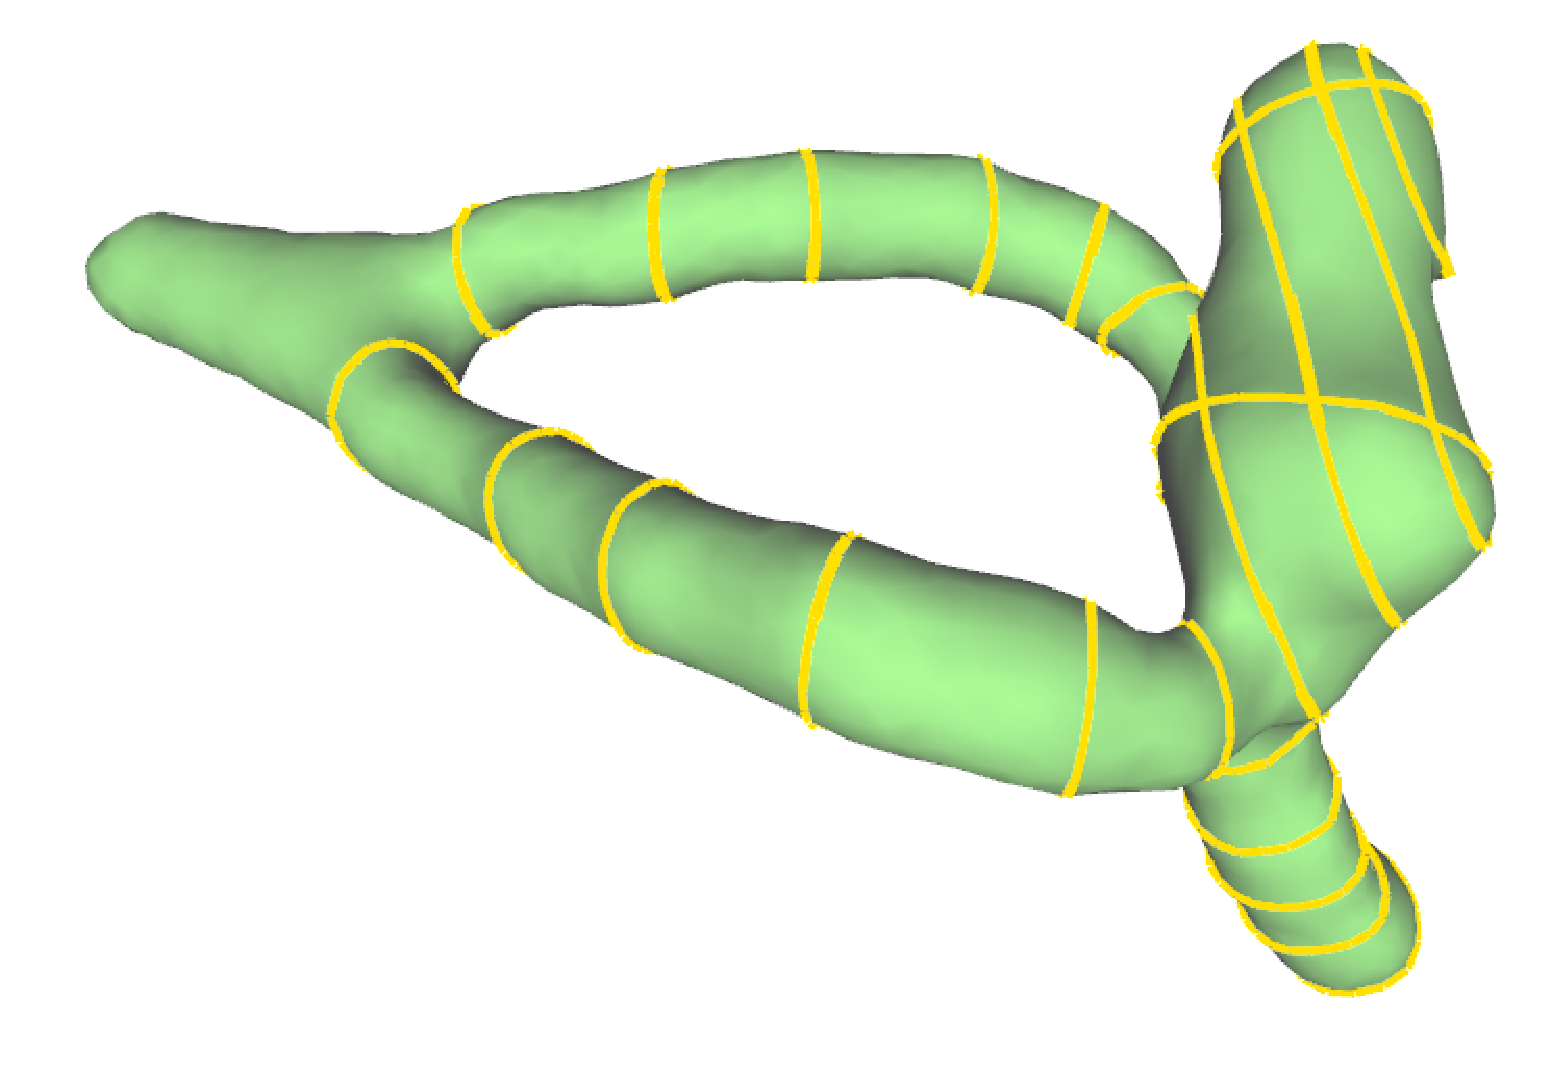
\includegraphics[scale=0.14]{figs/f6.anatomy-result-initial.eps}%0.15
    \end{minipage}}
  \subfigure[]{
    \label{fig:anatomy:d}
    \begin{minipage}[b]{0.23\textwidth}
      \centering
      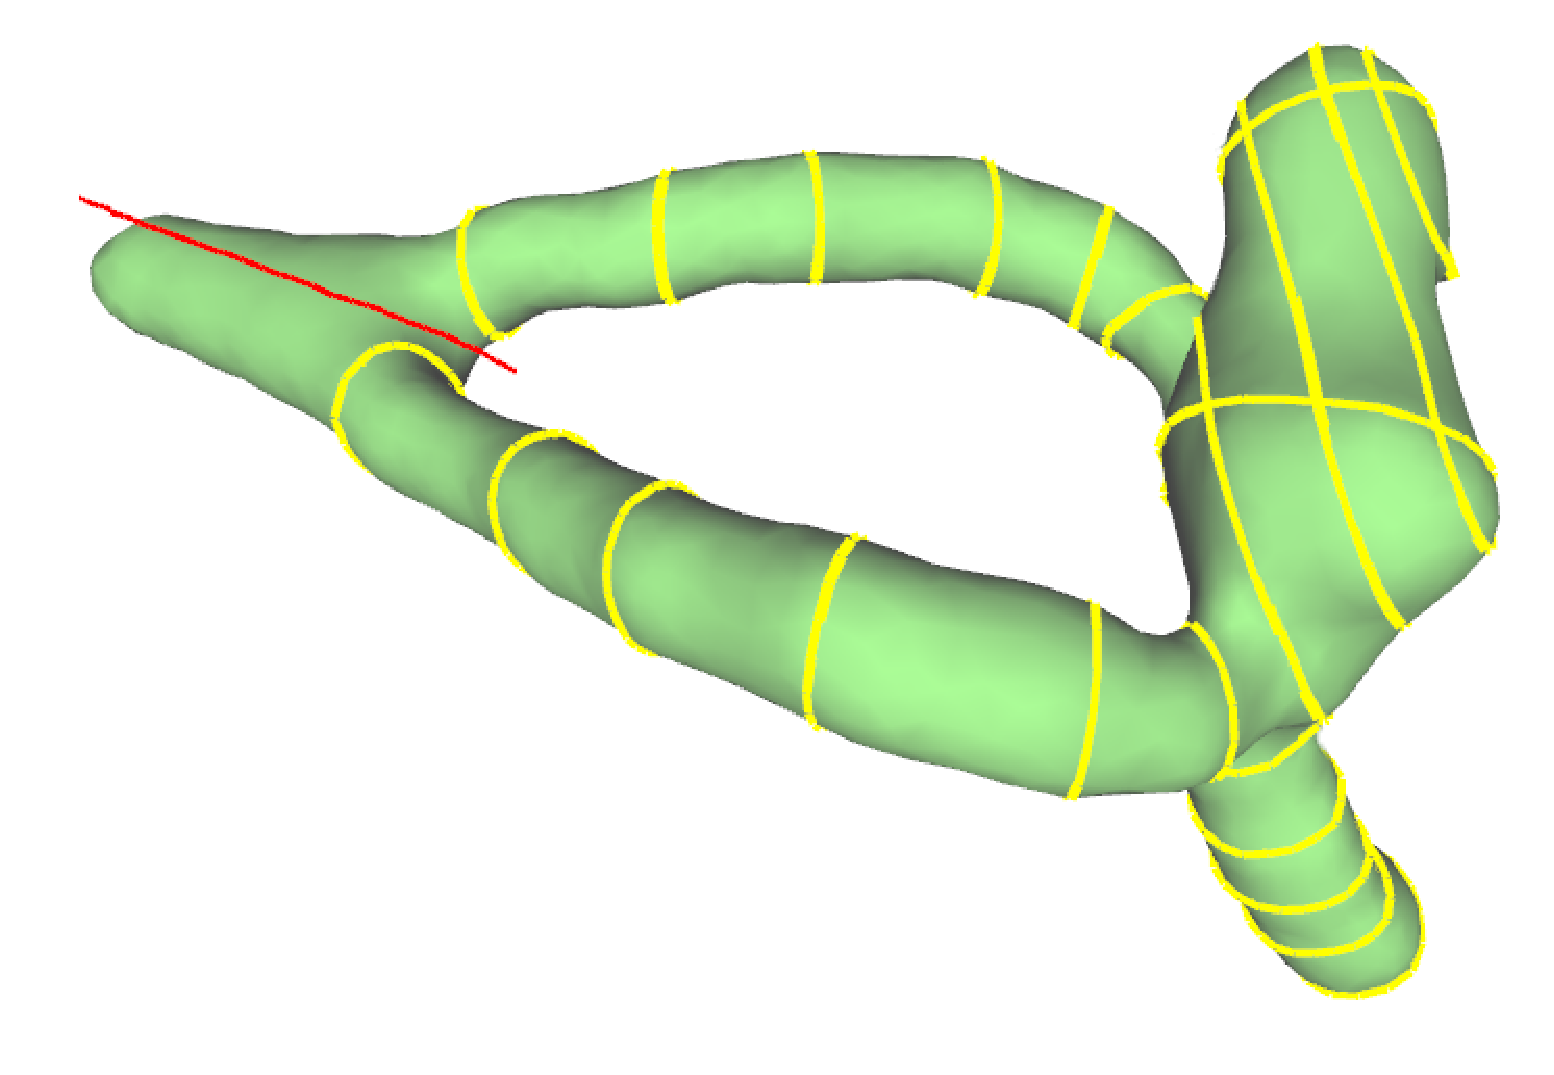
\includegraphics[scale=0.14]{figs/f6.anatomy-split.eps}%0.15
    \end{minipage}}
  \subfigure[]{
    \label{fig:anatomy:e}
    \begin{minipage}[b]{0.23\textwidth}
      \centering
      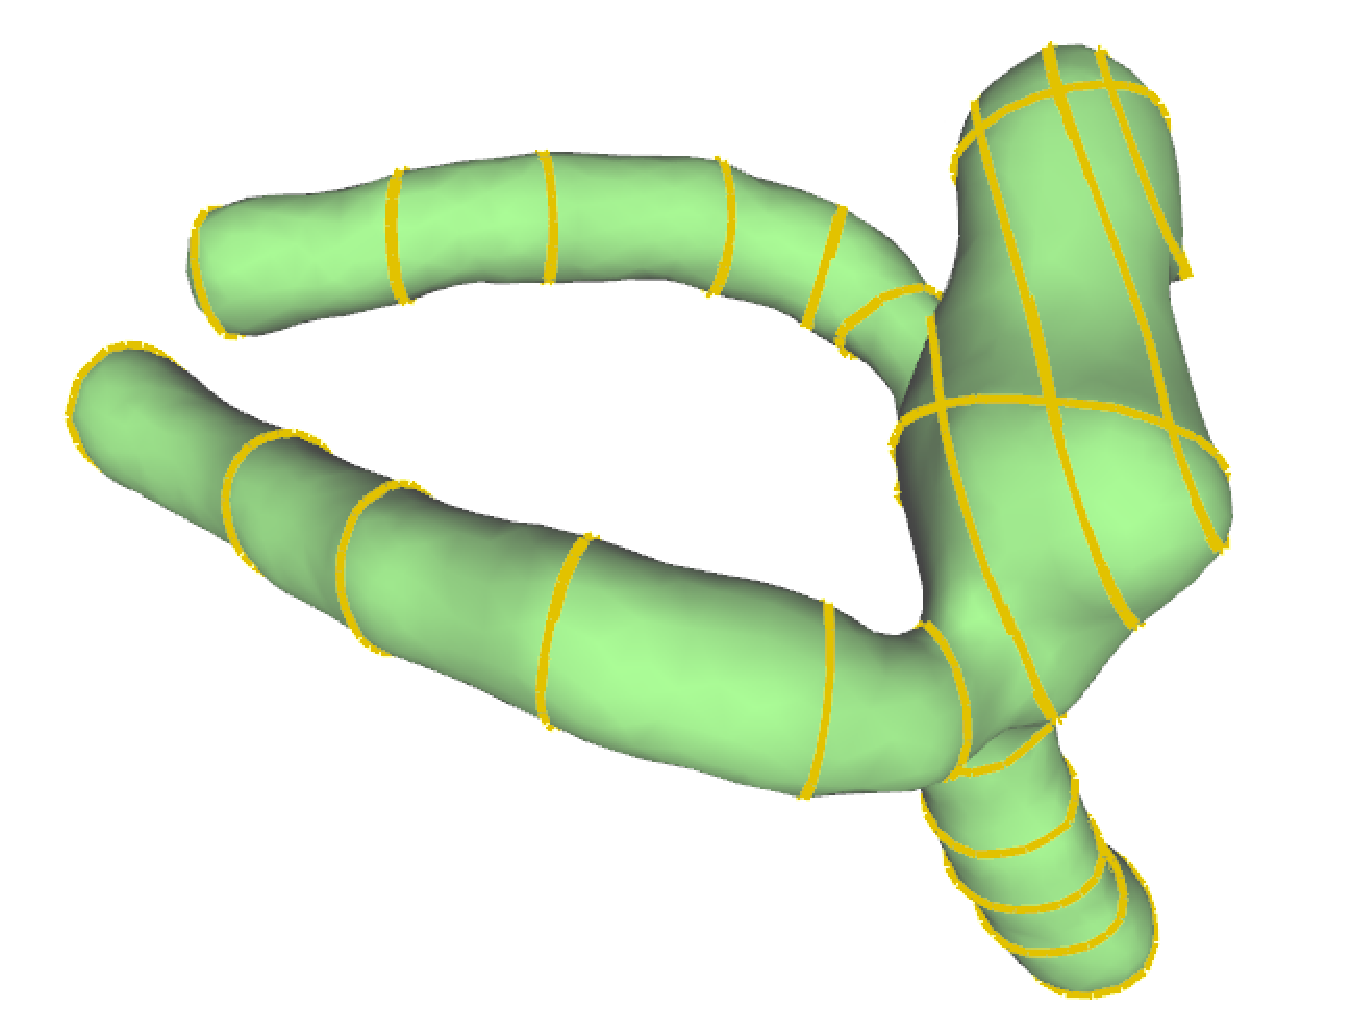
\includegraphics[scale=0.15]{figs/f6.anatomy-result-edited.eps}%0.16
    \end{minipage}}
  \caption{The proposed surface reconstruction process for the input cross sections given in Figure~\ref{fig:anatomy-ju}(a).
  (a) Reconstructed sub-surfaces in zones.
  (b) The reconstructed surface that has only one connected component.
  (c) Sketching a stroke (red) to indicate the local region to be split if desired.
  (d) The reconstructed result after splitting. }
  \label{fig:anatomy}
\end{figure*}

%our solution
To solve these problems,  we propose a new surface reconstruction
framework. First of all, we generalize the algorithm
proposed in Chapter~\ref{ch:orthsurf} to build a manifold surface interpolating the input cross section curves with arbitrary orientations. Generally, our method follows the same workflow to partition the whole 3D
space into zones and get the final surface by stitching the
sub-surfaces built inside each zone. However, we use more delicate methods for computing the sub-surface within each zone whose shape will be more complex and extending the surface components generated from some cross sections when necessary, such that regular local shapes can be produced and isolated surface parts can be effectively connected.

Moreover, we provide simple sketching tools to allow the further
modification of the topology of the reconstruction result, if the
user is not satisfactory with the initial shape. Different from
existing topology-editing approaches, our tools make use of the
intermediate calculation results obtained during the surface
reconstruction process, and avoid the global analysis and
processing of the 3D model from the beginning. Thus, the
reconstruction and modification of a desired surface will be carried out
in a consistent manner in our framework.

The most important feature of  our framework is that the output
surface is guaranteed to be a manifold surface having only one
connected component, which is usually consistent with the user's
expectation when reconstructing a 3D model from given cross
sections. Since our method is a local scheme, we are able to
implement the calculations of the sub-surfaces in all zones in
parallel to speed up the whole surface reconstruction process.
Figure~\ref{fig:anatomy} shows the reconstruction and editing of an
anatomy model in our framework, with comparison to the result of a
previous method~\cite{LBDLJ08}.

%organization
The rest of this chapter is organized as  follows:
Section~\ref{ch6:sec:ov} gives an overview of our surface
reconstruction framework. Section~\ref{ch6:sec:reconst} describes
the details of the generalized surface reconstruction algorithm. The
sketch-based topology editing of the reconstructed model, including
the user interface and algorithm, is provided in
Section~\ref{ch6:sec:edit}. The experimental results and analysis
are provided in Section~\ref{ch6:sec:result}.




%----------------------------------------------------------------------------
%\section{Prior Work}
%\label{sec:review}

%early works,one cross section per slice
%Early  works on mesh surface reconstruction~\cite{KE75, FKU77,
%CS78, Kd82, GD82, WA86} focus on handling the interpolation of
%parallel cross sections, for example, each of which lies on one
%slice of the medical data scanned using CT or other devices. In
%these works, strategies are proposed to find polygonal tiling
%between each pair of cross sections on neighboring slices. While
%for slices containing multiple cross sections, these methods do not
%work since it will be difficult to establish the correspondence
%between more than two cross sections on neighboring slices.

%parallel: triangulation
%To avoid the  disadvantages of the global approach,~\cite{BJ88,
%MSS92, GB93, FL98, CD99} used the triangulation methods to compute
%a volumetric mesh interpolating cross sections on each pair of
%planes, such that correspondence between the curves can be
%established and a surface mesh can be extracted. To avoid the
%complicated calculation in fitting a volumetric
%mesh,~\cite{BS96,BCL96,OPC96,KSS00,BGLS04,JWCET05,BV07} proposed to
%project the cross sections from neighboring planes onto a common
%plane and match the projections from different cross sections. The
%final surface can then be built by connecting the curves and their
%projections.

%parallel: implicit
%Subsequent  works proposed various solutions on handling more
%complicated cross sections on parallel planes. For examples, the
%works~\cite{HZB92, CNKG02, TO99} extended the implicit surface
%method which is often used in the point cloud fitting problem to
%fit an implicit function to the input curves, extract the
%isosurface and convert it to a mesh. Some works also considered the
%normal~\cite{BMSdV10} or material~\cite{WD00} constraints during
%the fitting process. However the global fitting method using
%implicit function may produce werid local shapes due to the
%sparsity of the cross section data. Tessellation of the isosurface
%should also be taken care of to make sure the final surface still
%interpolate the input curves, and the time for computation may be
%long.



%non-parallel
%There have also  been some attempts made to reconstruct surfaces
%from non-parallel cross sections.~\cite{RU90, WMTBDC95, BTS04}
%extended the implicit function method to build a surface composed
%of patches, each of which is bounded by cross sections on two
%adjacent planes.~\cite{PT94,DP97,BM07} used a divide-and-conquer
%scheme which first partitions the whole space into zones bounded by
%the planes that the cross sections lie on. Then within each zone,
%Delaunay triangulation is used to compute a sub-surface that
%connects the cross sections on the faces of the zones. The
%triangulation methods provide a feasible approach to build surfaces
%from non-intersected cross sections, while for those who have
%intersections or even more complex relationship, it will fail to
%produce a satisfactory result.

%A more recent  work~\cite{LBDLJ08} also adopted the
%divide-and-conquer scheme and extended the method in~\cite{JWCET05}
%to handle more complicated non-parallel cross sections. In each
%zone, the cross sections are projected onto the medial axis planes
%to establish the correspondence and sub-surface is built by
%connecting the cross sections and their projections. The quality of
%the final surface is then improved through iterative smoothing and
%refinement. This method has been used in the reconstruction of 3D
%medical data from contours of scanned 2D images~\cite{SLJGAGL09}.
%Although it can handle non-parallel cross sections with more
%complex relationship, the reconstruction result heavily relies on
%the geometric agency (i.e., the medial axis plane). When the shape
%of the zone becomes complex, the agency may become irregular,
%leading to unexpected topological noise to the result surface.

%local method: multi-component problem
%Meanwhile,  all these methods on handling the non-parallel cross
%sections aim at building a single object. They used a standard
%partition scheme in Computational Geometry to subdivide the 3D
%space into convex arrangements~\cite{BM07}. However, we will show
%in Section~\ref{sec:reconst} that this partition algorithm may
%separate the connections of different surface components. As a
%result, the final object will be composed of multiple disconnected
%components, while in most cases a one-component surface is desired.
%Contrarily,~\cite{EB11} proposed an approach to build multiple
%objects from multi-labeled contours at the same time instead of one
%single object, by defining rules to distinguish components
%belonging to different objects. Both self-intersections and
%inter-object intersections between these components can be avoided.
%While this is useful in some bio-medical modeling applications such
%as reconstructing neurons from electron microscopy images, the
%multi-component problem when building one single object still
%remains.

%post-edit after reconstruction
%Finally,  although all these algorithms focus on the reconstruction
%of 3D objects with satisfactory shapes, sometimes the topology of
%the result model still cannot meet the user's expectation. In that
%case, post-editing of the model is often needed, while these
%reconstruction algorithms can provide little useful information to
%this operation but only the 3D model itself. There have been some
%topology editing tools, especially those with simple sketch-based
%interfaces proposed~\cite{JZH07,JT09,HRABV11}. However, these
%methods all require to globally analyze and modify the model
%according to the user input, which seems complicated. In other
%words, the reconstruction and editing of the 3D model are regarded
%as independent operations. Our algorithm builds a bridge to connect
%them to help produce a 3D model with satisfactory shape in an
%efficient and natural manner.




%%-----------------------------------------------------------------------------
\section{Overview of the algorithm}
\label{ch6:sec:ov}

%problem description/statement
The input in our algorithm is a set  of cross sections
$CS=\{cs_i~|~i=1,...,m\}$ lying on \emph{arbitrary} planes
$P=\{p_i~|~i=1,...,n\}$ in 3D space $\mathbb{R}^3$. The cross
sections are closed curves represented as polylines. Similar to that
in Chapter~\ref{ch:orthsurf}, the output of this algorithm is  a
closed 2-manifold triangular mesh $M$ interpolating the input cross
sections $CS$ and having only one connected component.

%To make the output a valid manifold surface, there are some further constraints on the input cross sections. For example, cross sections on a same plane should not have intersections; The set of intersection points $\bigcap_{{p_i}{cs_j}}$ between plane $p_i$ and cross sections $cs_j$ on plane $p_j$ must be exactly the same as the set $\bigcap_{{p_j}{cs_i}}$ of $p_j$ and $cs_i$ on plane $p_i$. The inside/outside information of the target surface $M$ should be consistent with that of the $CS$, which can be deducted from their containing relationship. For the details of the restrictions on the cross sections and the deductions on the inside/outside information, please refer to Section~\ref{ch3:sec:algo:rule}.

Our method adopts  the same workflow in Chapter~\ref{ch:orthsurf} to
reconstruct surfaces from cross sections. That is, we first place a
large virtual bounding box outside all the cross sections. Here the
size of the box is set to 2 times that of the bounding box of all
points on the cross sections, and its shape may not be a cube as in
Chapter~\ref{ch:orthsurf}. Then we partition it into zones
$ZN=\{zn_i~|~i=1,...,m\}$ by using the planes that the cross
sections lie on. The curves are then put onto the faces
$F=\{f_{ij}~|~f_{ij}\in zn_i,j=1,...,n\}$ of each zone $zn_i$. Next
we build a sub-surface which interpolates the curves on the faces of
each zone and stitch all the pieces of sub-surfaces together to form
a complete surface. Finally we improve the quality of the mesh
surface through iterative refinement and smoothing.

Similar to  the algorithm in Chapter~\ref{ch:orthsurf}, we use the
CSG-based method to generate the sub-surface which interpolates
curves on the zone faces, such that a manifold surface with regular
local shapes can be reconstructed. We also extend the potentially
isolated surface components by adding some virtual cross sections,
to reduce the possibility of the existence of isolated surface
components. Comparing to the previous method~\cite{LBDLJ08}, our
approach does not rely on any geometric agency and can join adjacent
surface parts flexibly. What is more, the information obtained
during this process can be retained and further used for the
computation of topology editing of the reconstructed model, such
that complicated analysis and computation of the global surface in
topology editing operations can be avoided.

In next two sections, we describe the surface reconstruction
algorithm and the sketch-based topology editing approach in detail.



\section{Surface reconstruction}
\label{ch6:sec:reconst}

%goals for the surface reconstruction
A basic goal for sub-surface reconstruction is  to make the result
surface totally lie within the zone and interpolate the input curves
on its faces. We do not use any geometric agency (for example, the
medial axis plane in~\cite{LBDLJ08}) whose computation is sensitive
to the shape of the zone to avoid creating artifacts. Meanwhile, it
would be better if the scheme is re-configurable, to make the
topology of the local surface more flexible to adjust when the
initial result is not satisfactory.

%2d illustration of surface reconstruction
\begin{figure*} [htbp]
  \centering
  \subfigure[]{
    \centering
    \label{fig:workflow2d:a}
    \begin{minipage}[b]{0.23\textwidth}
      \centering
      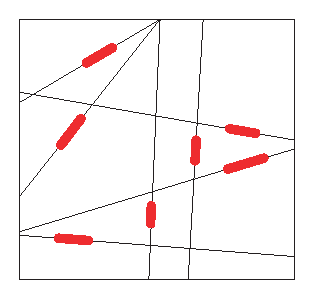
\includegraphics[scale=0.6]{figs/f6.illu-workflow-2d1.eps}
    \end{minipage}}
  \subfigure[]{
    \centering
    \label{fig:workflow2d:b}
    \begin{minipage}[b]{0.23\textwidth}
      \centering
      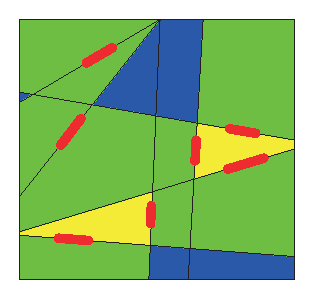
\includegraphics[scale=0.6]{figs/f6.illu-workflow-2d2.eps}
    \end{minipage}}
  \subfigure[]{
    \label{fig:workflow2d:c}
    \begin{minipage}[b]{0.23\textwidth}
      \centering
      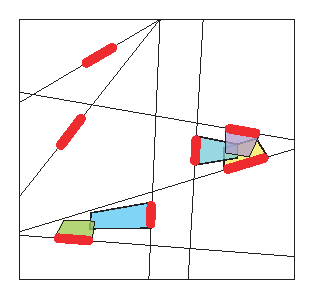
\includegraphics[scale=0.6]{figs/f6.illu-workflow-2d3.eps}
    \end{minipage}}
  \subfigure[]{
    \label{fig:workflow2d:d}
    \begin{minipage}[b]{0.23\textwidth}
      \centering
      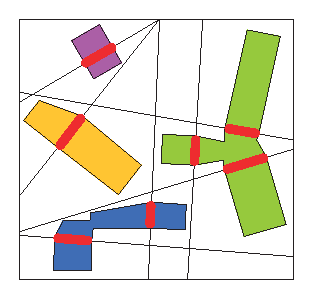
\includegraphics[scale=0.6]{figs/f6.illu-workflow-2d4.eps}
    \end{minipage}}
  \subfigure[]{
    \label{fig:workflow2d:e}
    \begin{minipage}[b]{0.23\textwidth}
      \centering
      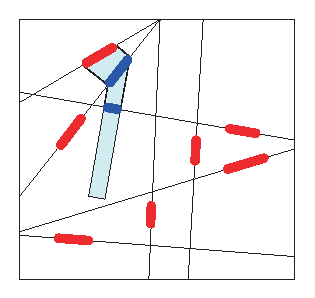
\includegraphics[scale=0.6]{figs/f6.illu-workflow-2d5.eps}
    \end{minipage}}
  \subfigure[]{
    \label{fig:workflow2d:f}
    \begin{minipage}[b]{0.23\textwidth}
      \centering
      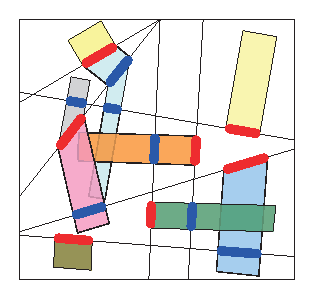
\includegraphics[scale=0.6]{figs/f6.illu-workflow-2d6.eps}
    \end{minipage}}
  \subfigure[]{
    \label{fig:workflow2d:g}
    \begin{minipage}[b]{0.23\textwidth}
      \centering
      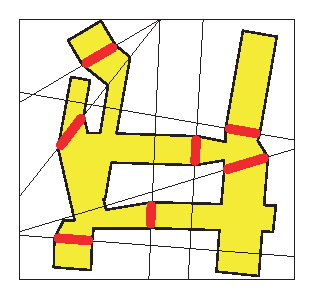
\includegraphics[scale=0.6]{figs/f6.illu-workflow-2d7.eps}
    \end{minipage}}
  \caption{2D illustration of our surface reconstruction algorithm.
  (a) Input segments (red, corresponding to the 3D cross sections) and partitioned zones.
  (b) The \textit{empty} zones (blue), \textit{end} zones (green) and \textit{body} zones (yellow).
  (c) Generating polygons (corresponding to the frusta) in \textit{body} zones.
  (d) Generating polygons in the \textit{end} zones using the same way as the reconstruction in the \textit{body} zones. The reconstruction result contains multiple components.
  (e) Generating extended polygons for an \textit{end} zone. The blue segments correspond to the virtual cross sections we built.
  (f) Generating polygons for all \textit{end} zones.
  (g) The reconstruction result. }
  \label{fig:workflow2d}
\end{figure*}

%inspiration of the method
To achieve these goals, we first use the strategy in
Chapter~\ref{ch:orthsurf} to partition zones into three types: the
\textit{empty} zone which has no faces containing cross sections,
the \textit{end} zone with only one face containing cross sections,
and the \textit{body} zone with two or more faces containing cross
sections. A 2D illustration of the partition result and zone types
can be found in Figure~\ref{fig:workflow2d}, in which the segments
on the lines correspond to the cross sections on the zone faces.

However, different from the case in  Chapter~\ref{ch:orthsurf}, the
shape of each zone is generally not a cuboid. As a result, the
method on generating the cylinders cannot be simply used since it is
difficult to ensure that the built cylinders lie within the zone. So
here for each cross section $cs_p$ in zone $zn_i$, we build a
frustum, instead of a cylinder, as the generated sub-surface
interpolating $cs_p$ in $zn_i$ and then compute the union of these
frusta. The surface of the result solid is then taken as the
sub-surface computed in $zn_i$, and all the pieces of sub-surfaces
are stitched together to form the global surface.



\subsection{Sub-surface reconstruction for a \textit{body} zone}
\label{ch6:sec:reconst:body}

In a \textit{body} zone, each cross  section may either intersect
with another cross section on a different face or not. Depending on
this intersection relationship, different strategies are adopted to
create the frustum from each cross section.

%create frustum from non-intersected cross sections
%illustration on sub-surface generation for non-intersected case
\begin{figure} [htbp]
  \centering
  \subfigure[]{
    \centering
    \label{fig:frunonint:a} %% label for first subfigure
    \begin{minipage}[b]{0.3\textwidth}%\textwidth   %\linewidth
      \centering
      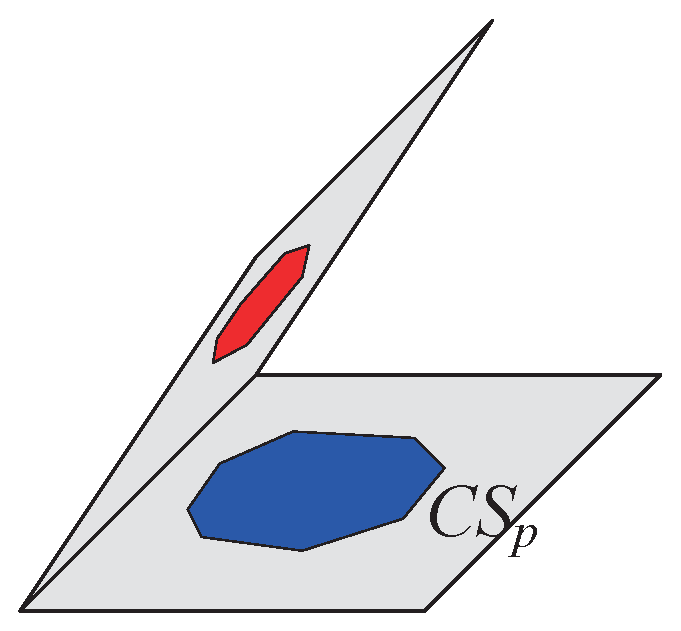
\includegraphics[scale=0.28]{figs/f6.illu-fru-non-intsct1.eps}%0.25
    \end{minipage}}
  \subfigure[]{
    \centering
    \label{fig:frunonint:b}
    \begin{minipage}[b]{0.3\textwidth}
      \centering
      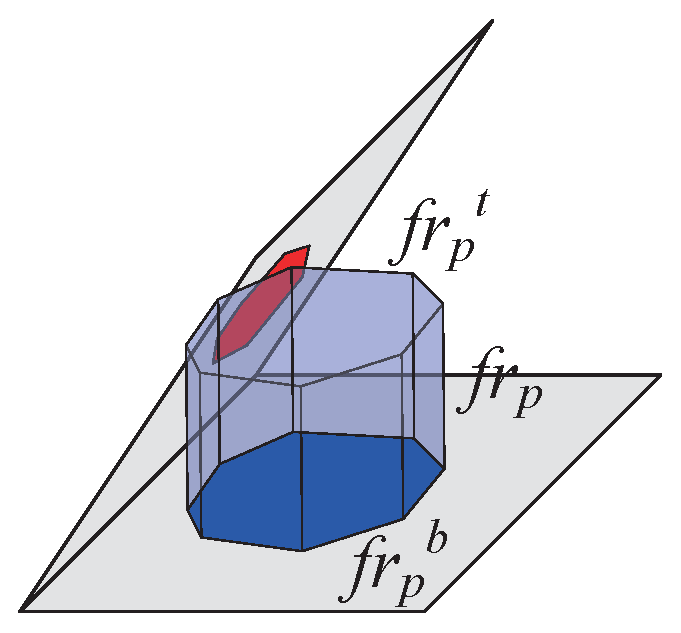
\includegraphics[scale=0.28]{figs/f6.illu-fru-non-intsct2.eps}
    \end{minipage}}
  \subfigure[]{
    \label{fig:frunonint:c}
    \begin{minipage}[b]{0.3\textwidth}
      \centering
      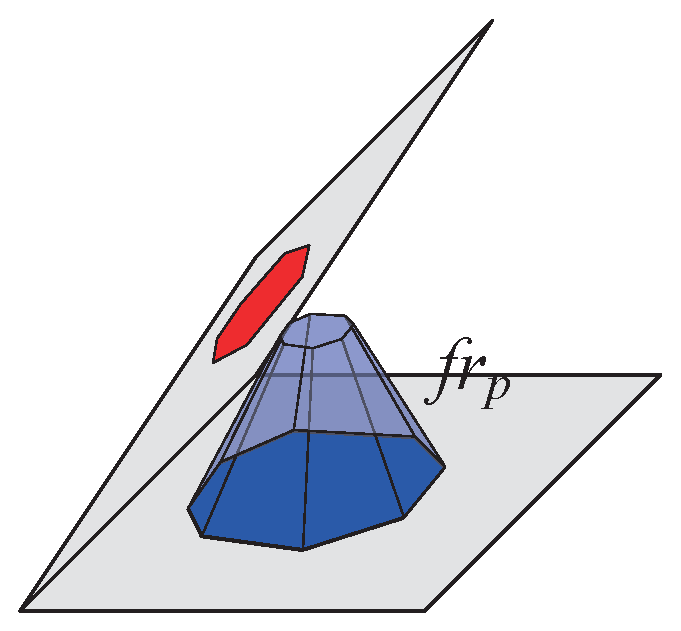
\includegraphics[scale=0.28]{figs/f6.illu-fru-non-intsct3.eps}
    \end{minipage}}
  \subfigure[]{
    \centering
    \label{fig:frunonint:d}
    \begin{minipage}[b]{0.3\textwidth}
      \centering
      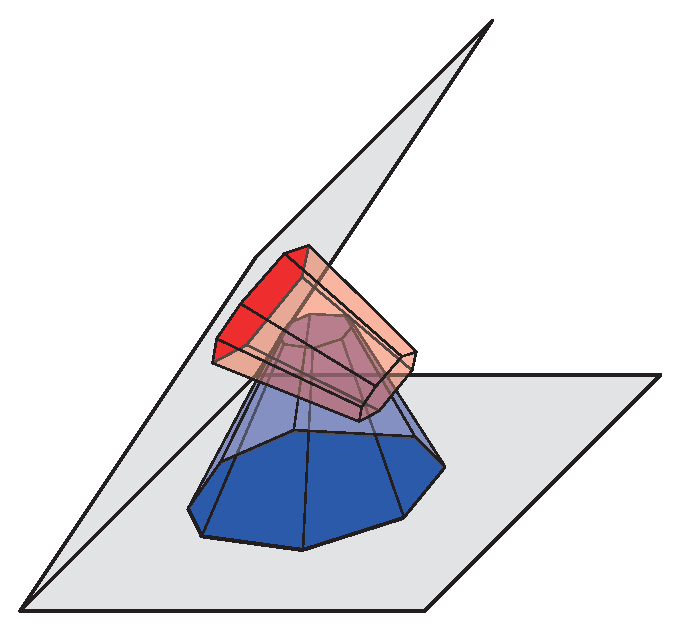
\includegraphics[scale=0.28]{figs/f6.illu-fru-non-intsct4.eps}
    \end{minipage}}
  \subfigure[]{
    \centering
    \label{fig:frunonint:e}
    \begin{minipage}[b]{0.3\textwidth}
      \centering
      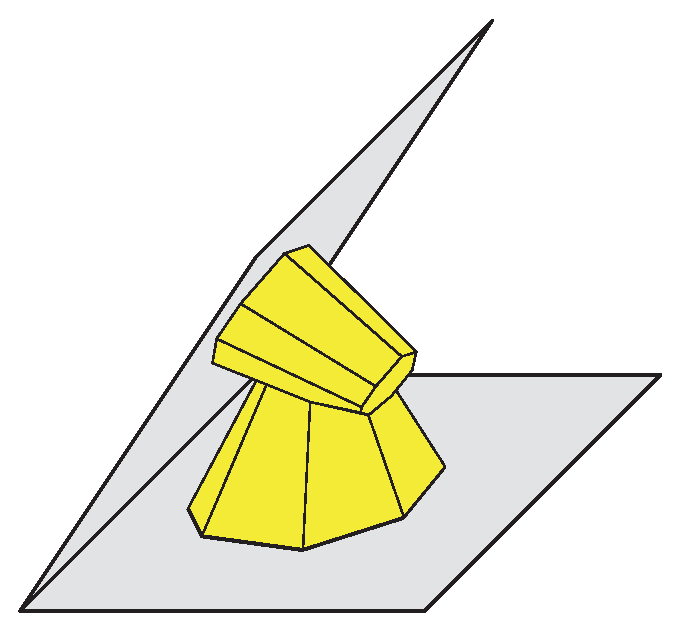
\includegraphics[scale=0.28]{figs/f6.illu-fru-non-intsct5.eps}
    \end{minipage}}
  \caption{Illustration of sub-surface reconstruction for non-intersected cross sections in a \textit{body} zone.
  (a) Input cross sections.
  (b) Generate initial frustum $fr_p$ from one cross section.
  (c) Adjust the top $fr_p^t$ of the frustum to make it lie within the zone.
  (d)Generate another frustum.
  (e) Compute the union of the two frusta.}
  \label{fig:frunonint}
\end{figure}

\textbf{Case 1}: For a cross section $cs_p$ on face $f_{ij}$ which
does not intersect with other cross sections in zone $zn_i$ (see
Figure~\ref{fig:frunonint:a}), we need to build a frustum $fr_p$
taking the 2D region enclosed by $cs_p$ as the bottom $fr_p^b$. The
initial top $fr_p^t$ of $fr_p$ is obtained by translating $fr_p^b$
along the direction orthogonal to $f_{ij}$ and pointing towards the
inside of $zn_i$. To get the distance of this translation (i.e. the
initial height value $h_p$ for the frustum), we compute a ray
starting from the center of $fr_p^b$ and pointing towards the inside
of $zn_i$ with the directions orthogonal to $f_{ij}$. The ray will
intersect with the other faces of $zn_i$ and the nearest
intersection point to the center of $fr_p^b$ is selected. Suppose
the distance between these two points is $d_p$, then the height will
be computed as:

\begin{equation}
\label{eq:frheight}
h_p = d_p- \epsilon,
\end{equation}
where $\epsilon$ is a small positive number to make sure that the
center of $fr_p^t$ lie within $zn_i$. Then if there are any points
on $fr_p^t$ lying outside $zn_i$ (see Figure~\ref{fig:frunonint:b}),
we keep shrinking $fr_p^t$ towards its center until $fr_p^t$ locates
totally inside of $zn_i$ or a predefined shrinkage ratio is reached
(see Figure~\ref{fig:frunonint:c}). If the latter happens, we
iteratively decrease the height value $h_p$ and re-compute $fr_p^t$
in this method until $fr_p$ totally lies inside $zn_i$. We do not
allow $fr_p^t$ to shrink to a single point to avoid making $fr_p$ a
cone which may cause numerical issues in the subsequent union
calculation. It can be seen that this method is simple and quick to
construct a frustum which is guaranteed to lie totally within the
zone and interpolate the cross section.


%create frustum from intersected cross sections
%illustration on sub-surface generation for intersected case
\begin{figure} [htbp]
  \centering
  \subfigure[]{
    \centering
    \label{fig:fruint:a} %% label for first subfigure
    \begin{minipage}[b]{0.23\textwidth}%\textwidth   %\linewidth
      \centering
      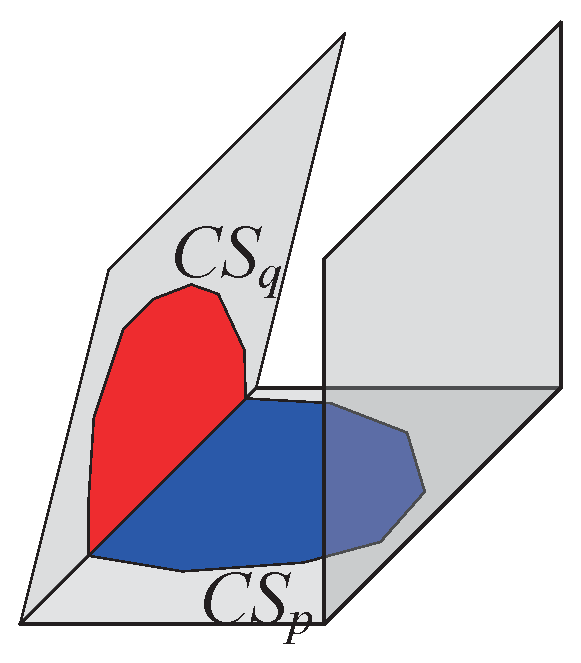
\includegraphics[scale=0.25]{figs/f6.illu-fru-intsct1.eps}%0.2
    \end{minipage}}
  \subfigure[]{
    \centering
    \label{fig:fruint:b}
    \begin{minipage}[b]{0.23\textwidth}
      \centering
      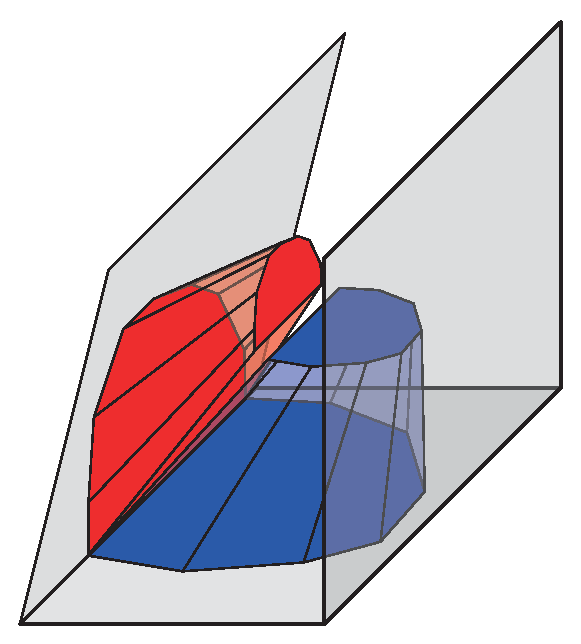
\includegraphics[scale=0.25]{figs/f6.illu-fru-intsct2.eps}
    \end{minipage}}
  \subfigure[]{
    \label{fig:fruint:c}
    \begin{minipage}[b]{0.23\textwidth}
      \centering
      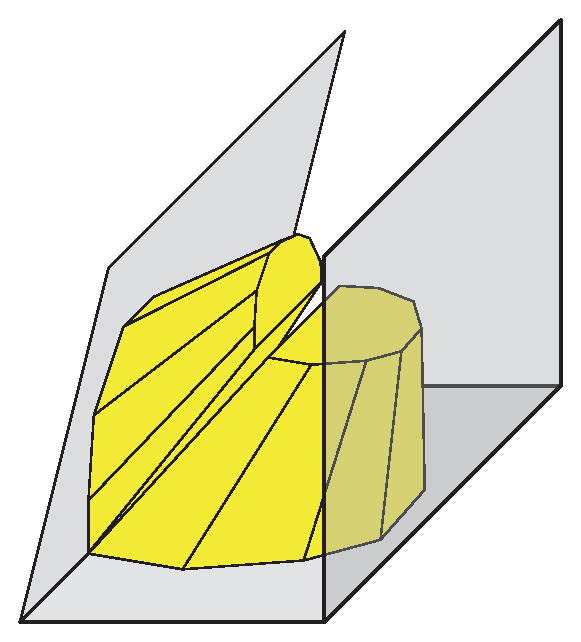
\includegraphics[scale=0.25]{figs/f6.illu-fru-intsct3.eps}
    \end{minipage}}
  \subfigure[]{
    \centering
    \label{fig:fruint:d}
    \begin{minipage}[b]{0.23\textwidth}
      \centering
      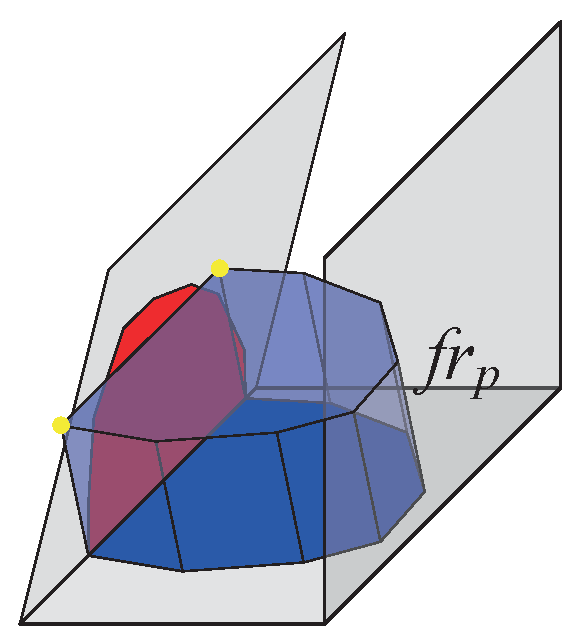
\includegraphics[scale=0.25]{figs/f6.illu-fru-intsct4.eps}
    \end{minipage}}
  \subfigure[]{
    \centering
    \label{fig:fruint:e}
    \begin{minipage}[b]{0.23\textwidth}
      \centering
      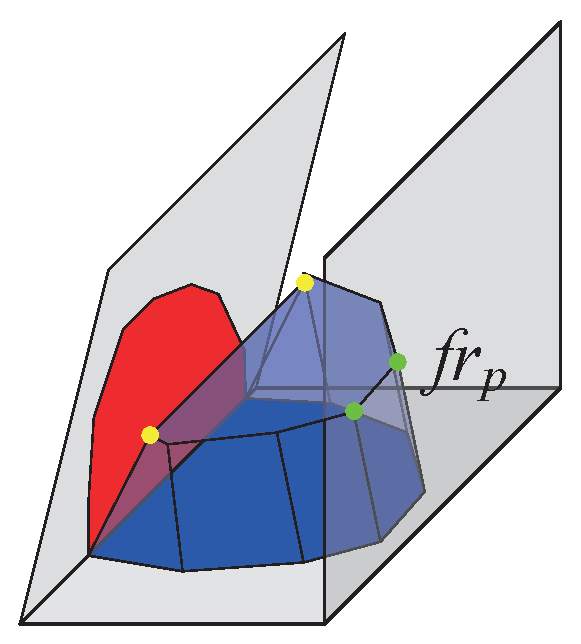
\includegraphics[scale=0.25]{figs/f6.illu-fru-intsct5.eps}
    \end{minipage}}
  \subfigure[]{
    \centering
    \label{fig:fruint:f}
    \begin{minipage}[b]{0.23\textwidth}
      \centering
      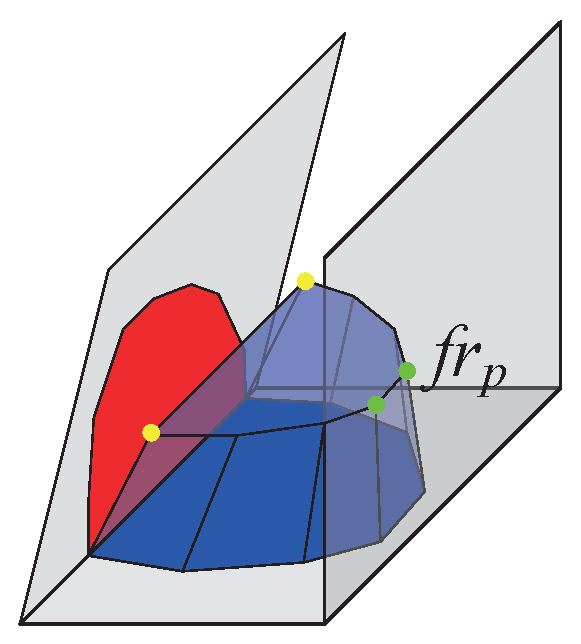
\includegraphics[scale=0.25]{figs/f6.illu-fru-intsct6.eps}
    \end{minipage}}
  \subfigure[]{
    \centering
    \label{fig:fruint:g}
    \begin{minipage}[b]{0.23\textwidth}
      \centering
      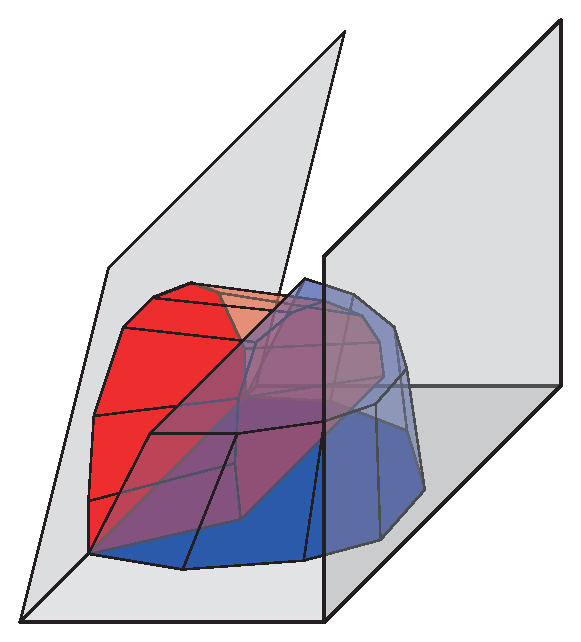
\includegraphics[scale=0.25]{figs/f6.illu-fru-intsct7.eps}
    \end{minipage}}
  \subfigure[]{
    \centering
    \label{fig:fruint:h}
    \begin{minipage}[b]{0.23\textwidth}
      \centering
      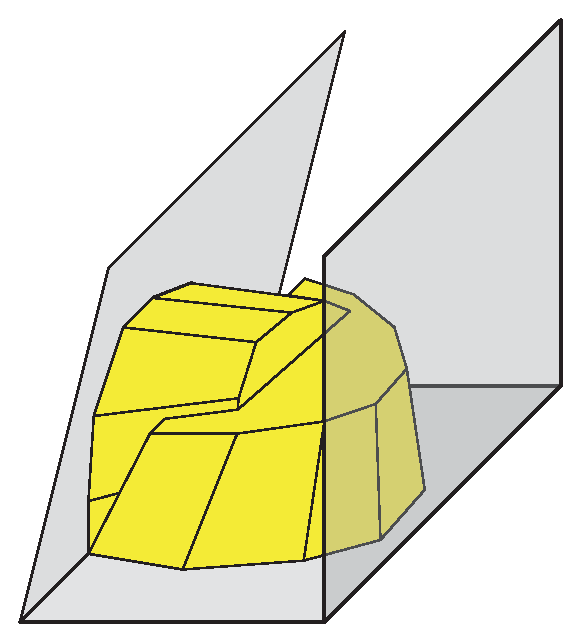
\includegraphics[scale=0.25]{figs/f6.illu-fru-intsct8.eps}
    \end{minipage}}
  \caption{Illustration of sub-surface reconstruction for intersected cross sections in a \textit{body} zone.
  (a) Input cross sections.
  (b) Generate the frusta by shrinking the top faces.
  (c) Non-manifold sub-surface caused by the over-shrinkage of the top of each frustum.
  (d) Translate the bottom $fr_p^b$ to get the initial frustum $fr_p$. The yellow dots represent the points outside the zone (i.e. $PT_f$ in Eq~\ref{eq:curvedeform2}).
  (e) Move the outside points into the zone. The green dots are the points near the other faces of the zone (i.e. $PT_o$ in Eq~\ref{eq:curvedeform2}).
  (f) Deform the boundary of the frustum top by keeping the yellow and green points fixed, to get a valid frustum.
  (g) Generate another frustum.
  (h) Compute the union of the two frusta.}
  \label{fig:fruint}
\end{figure}

\textbf{Case 2}: When  a cross section $cs_p$ on face $f_{ij}$
intersects with another cross section $cs_q$ on the neighbor face
$f_{ik}$ of $f_{ij}$ in zone $zn_i$ (see Figure~\ref{fig:fruint:a}),
the goal of the sub-surface reconstruction is to make sure that
$fr_p$ and $fr_q$ (frusta generated from $cs_p$ and $cs_q$
respectively) lie within $zn_i$ and intersect with each other on
more than the common segment of $cs_p$ and $cs_q$, such that the
surface of their union is a closed manifold that interpolates both
the two cross sections. In that case, the bottom $fr_p^b$ is simply
taken as the region enclosed by $cs_p$ and the edges of $f_{ij}$,
but the computation of the top $fr_p^t$ will be more involved.
Especially when the dihedral angle between $f_{ij}$ and $f_{ik}$ is
equal to or less than $\pi/2$, simple translation of $fr_p^b$ along
the orthogonal direction will make $cs_q$ covered by $fr_p^t$ (see
Figure~\ref{fig:fruint:d}) and the union result will not interpolate
$cs_q$, while over-shrinking $fr_p^t$ like the way we handle Case 1
may make the union result a non-manifold surface (see
Figure~\ref{fig:fruint:b} and~\ref{fig:fruint:c}).

Here we first adopt  the same method in handling Case 1 to get the
initial height value $h_p$ and the top $fr_p^t$ of $fr_p$.
Especially, we select the points on $fr_p^b$ whose distances to
$f_{ik}$ are smaller than a given threshold and mark their
corresponding points $PT_f$ on $fr_p^t$ (the yellow points in
Figure~\ref{fig:fruint:d}). These points are supposed to stay near
$f_{ik}$ inside $zn_i$ to make the union of $fr_p$ and $fr_p$ be a
valid solid whose surface is a manifold. Then we check if there
exist any points on $fr_p^t$ lying outside $zn_i$. If yes, we
translate them towards the center of $fr_p^t$ until they just get
inside of $zn_i$ (see Figure~\ref{fig:fruint:e}). Next, to preserve
the original shape of $fr_p^t$ and avoid undesired artifacts caused
by the translation of these points, we launch a deformation process
to deform the boundary curve $PT_b$ of $fr_p^t$. Specifically, we
try to fix the positions of $PT_f$ and preserve the Laplacian
vectors which are used to represent the local shape of the original
curve.
The Laplacian vector $\delta_i$ at each boundary points $pt_i$
of the initially obtained $fr_p^t$ can be calculated by using
Eq.~\ref{eq:curveLap}.

%%%%%%%%%%%%%%%%%%%%%%%%%%%%%%%%%%%%%%%%%%%%%%%%%
%%%%%%%%%deleted in thesis only, since has been introduced in Chapter 3
%The Laplacian vector $\delta_i$ is calculated at each
%boundary points $pt_i$ of the initially obtained $fr_p^t$, by using
%the equation:
%
%\begin{equation}
%\label{eq:curveLap}
%\delta_i=L(pt_i)=\frac{1}{N}\sum\limits_{j\in N(i)}{(pt_i-pt_j)},
%\end{equation}
%where $L(\cdot)$ is the Laplacian operator and $\{pt_j, j\in N(i)\}$ are the positions of the two neighboring points of $pt_i$.
%%%%%%%%%deleted in thesis only, since has been introduced in Chapter 3
%%%%%%%%%%%%%%%%%%%%%%%%%%%%%%%%%%%%%%%%%%%%%%%%%


We also fix the positions of points $PT_o$ which stay near the other
faces of $zn_i$ (the green points in Figure~\ref{fig:fruint:e}), to prevent
them from getting out of $zn_i$ after the deformation. So the total energy
to minimize for the deformation is:

\begin{eqnarray}
\label{eq:curvedeform2}
E(PT_b^\prime) &=& \sum\limits_{pt_i \in PT_b} {||L(pt_i^\prime)- T_i\delta_i||^2}+\nonumber\\
& & \sum\limits_{pt_i \in PT_f}{||pt_i^\prime-pt_i||^2}+\nonumber\\
& & \sum\limits_{pt_i \in PT_o}{||pt_i^\prime-pt_i||^2},
\end{eqnarray}
where $pt_i$ and $pt_i^\prime$ represent the original and deformed point positions.
$T_i$ denotes the transformation matrix of the Laplacian vector.
This curve deformation problem can then be solved by using the same method
we have introduced in Section~\ref{ch3:sec:algo:rule}.

%%%%%%%%%%%%%%%%%%%%%%%%%%%%%%%%%%%%%%%%%%%%%%%%%
%%%%%%%%%deleted in thesis only, since has been introduced in Chapter 3
%$T_i$ denotes the transformation matrix of the Laplacian vector whose calculation can be found in~\cite{ESA07}. Since all the points of $PT$ lie on the same plane, this is actually a 2D curve deformation problem that is easy to solve.
%%%%%%%%%deleted in thesis only, since has been introduced in Chapter 3
%%%%%%%%%%%%%%%%%%%%%%%%%%%%%%%%%%%%%%%%%%%%%%%%%


Although we tried to  anchor the points near the boundary faces of
$zn_i$, there may still exist some other points staying outside
$zn_i$ after the deformation. In that case, these points are then
translated towards the center of the deformed curve $PT_b$ until
they come into the inside of $zn_i$ and the set $PT_o$ will be
updated accordingly. After a few iterations of using
Eq.~\ref{eq:curvedeform2}, all points on $PT_b$ will be inside $zn_i$
and valid $fr_p$ can then be obtained (see
Figure~\ref{fig:fruint:f}). This method also works when $cs_p$
intersects with multiple cross sections.



\subsection{Sub-surface reconstruction for an \textit{end} zone}
\label{ch6:sec:reconst:end}

%why previous method does not work
It has been  introduced in Chapter~\ref{ch:orthsurf} that without
extension, the sub-surfaces generated in the \textit{end} zones may
probably become isolated and the whole surface will contain multiple
components. This may also happen for cross sections with arbitrary
orientations (see Figure~\ref{fig:workflow2d:d}). However, since the
shape of each zone may not be a cuboid,  the neighbor zone to extend
the frustum to should be carefully selected. The simple method of
extending in the orthogonal direction in Chapter~\ref{ch:orthsurf}
needs to be improved.

Here we adopt a new strategy to extend  the surface parts generated
from cross sections in the \textit{end} zones to non-end zones by
adding some virtual cross sections such that their possibility of
becoming disconnected surface parts will be minimized.

%illustration on sub-surface generation in an end zone
\begin{figure} [htbp]
  \centering
  \subfigure[]{
    \centering
    \label{fig:fruend:a} %% label for first subfigure
    \begin{minipage}[b]{0.4\textwidth}%\textwidth %0.46  %\linewidth
      \centering
      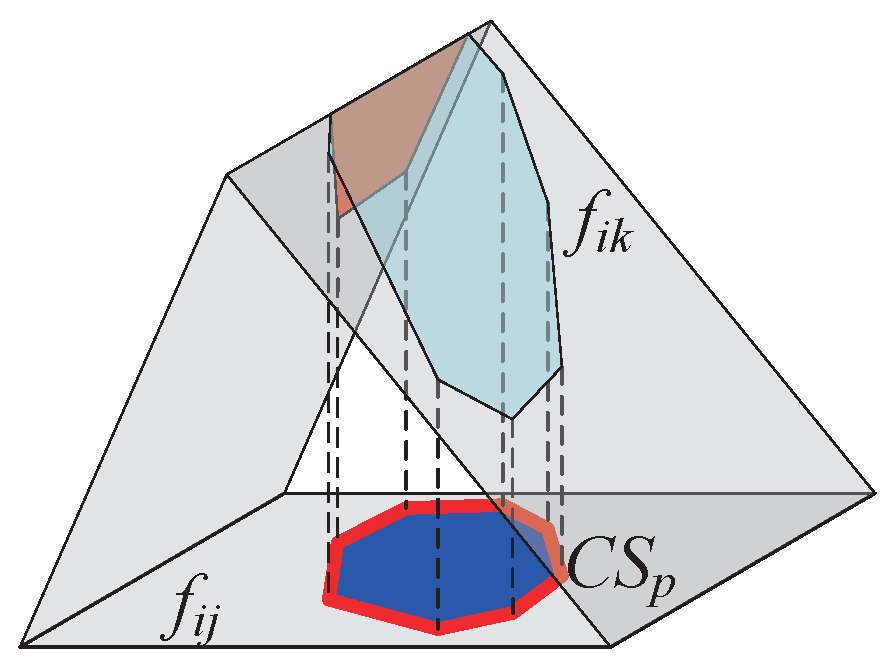
\includegraphics[scale=0.25]{figs/f6.illu-fru-endzone1.eps}%0.2
    \end{minipage}}
  \subfigure[]{
    \centering
    \label{fig:fruend:b}
    \begin{minipage}[b]{0.4\textwidth}
      \centering
      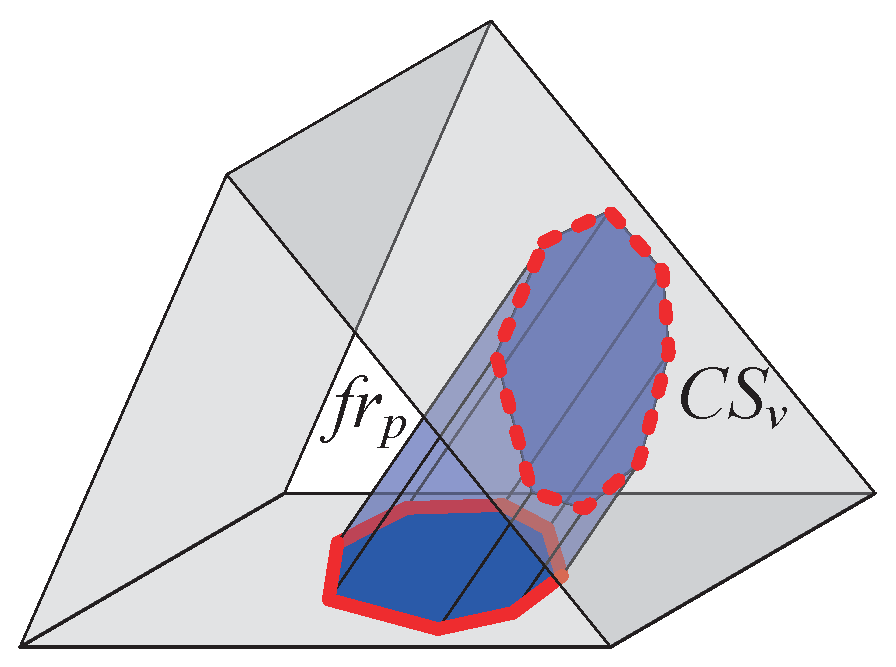
\includegraphics[scale=0.25]{figs/f6.illu-fru-endzone2.eps}
    \end{minipage}}
  \caption{Illustration of sub-surface reconstruction in an \textit{end} zone.
  (a) The input cross section $cs_p$ on face $f_{ij}$ is projected onto the other faces in the orthogonal direction of $f_{ij}$ and the face $f_{ik}$ with the largest projection area is selected.
  (b) A virtual cross section $cs_v$ is obtained by projecting $cs_p$ onto $f_{ik}$ and the frustum $fr_p$ is built by taking $cs_p$ and $cs_v$ as the bottom and top. }
  \label{fig:fruend}
\end{figure}

Specifically, for  each cross sections $cs_p$ on face $f_{ij}$ in an
\textit{end} zone $zn_i$, we build a frustum $fr_p$ taking the 2D
region enclosed by $cs_p$ as the bottom $fr_p^b$. Different from the
methods in Section~\ref{ch6:sec:reconst:body}, we check if the top
$fr_p^t$ of $fr_p$ can be built on another face $f_{ik}$ of the
zone, such that the surface components generated from $cs_p$ can be
easily extended to other zones. To do that, we project $fr_p^b$ onto
other faces of the zone in the direction orthogonal to $f_{ij}$, and
the face with the largest projection area will be selected as
$f_{ik}$ (see Figure~\ref{fig:fruend:a}). If $f_{ik}$ belongs to the
bounding box, then the extension will be considered as impossible
and the frustum will be built just in the method we handle Case 1 in
a \textit{body} zone, and this frustum will be treated as the
surface component generated from $cs_p$.

If $f_{ik}$ does not belong to the bounding box, the extension is
regarded as possible. In that case, to get the initial top $fr_p^t$,
$fr_p^b$ will be projected onto the plane that $f_{ik}$ lies on
along the direction orthogonal to the plane. If there are any points
of $fr_p^t$ lying outside $f_{ik}$, we just shrink $fr_p^t$ towards
its center until $fr_p^t$ is completely bounded by $f_{ik}$. By
connecting the corresponding points on $fr_p^b$ and $fr_p^t$, the
frustum in $zn_i$ can be built (see Figure~\ref{fig:fruend:b}).
Next, we take the boundary curve of $fr_p^t$ as a virtual cross
section $cs_v$ and continue building a new frustum from $cs_v$ in
the other zone $zn_k$ incident to face $f_{ik}$, by using the same
method as above. This process continues until the new face for
projecting the virtual cross section belongs to the bounding box, or
the next zone is a \textit{body} zone, and the method of handling
Case 1 in a \textit{body} zone will be used to generate the last
frustum. Finally, all the connected frusta which are created during
this process will be taken as the surface components generated from
the cross section $cs_p$.

By adding the  virtual cross sections and extending the frusta, the
possibly isolated surface components in the \textit{end} zones can
be effectively connected to other components in most cases, since
there is a very low possibility that all their extensions end up at
the boundary faces. Thus, the possibility of existence of multiple
components in a reconstructed model will be minimized. Since this
process starts from each \textit{end} zone simultaneously and
independently, the reconstruction result will be unique.

It has been mentioned  in Chapter~\ref{ch:orthsurf} that another
reason that causes the multi-component problem is that the
sub-surfaces generated from different cross sections in a
\textit{body} zone may not intersect with each other. In this
reconstruction scheme, it can be solved by changing the shape and
orientation of the frusta to force them intersect, which is easy to
do in a convex zone. However, we do not make that compulsory since
it may cause irregular local shapes and undesired connections. As we
will show in the next section, we give this freedom to the users to
allow them join these components by sketching a simple curve if
needed.



\subsection{Global surface reconstruction}
\label{ch6:sec:reconst:global}

Similar to Chapter~\ref{ch:orthsurf},  we use the algorithm proposed
in~\cite{LTH86} to compute the union of the generated frusta. Since
the frusta are simple shapes, this method is fast and robust enough
for our application. The calculation of the global surface
$M_{init}$ can be expressed as:

\begin{equation}
\label{eq:surfreconst}
%    M_{init}=\sum\limits_{i=1}^m {(fr_{i1} \bigcup fr_{i2} \bigcup {...} \bigcup fr_{in})},
    M_{init}=\sum\limits_{i=1}^m {(\bigcup\limits_{j = 1}^n {fr_{ij}})},
\end{equation}
in which $fr_{ij}$ refers to the  $j$th frustum built in zone
$zn_i$, assuming there are totally $m$ zones and $n$ frusta in each
zone. After the computation, all $fr_{ij}$ and their unions will
be preserved for the further edit operation if necessary, which will
be introduced in detail in Section~\ref{ch6:sec:edit}. Finally, we
iteratively refine and smooth the mesh surface using the same
algorithms adopted in Chapter~\ref{ch:orthsurf}.

It can be seen that in our  approach, the reconstruction result
directly depends on the primitives generated in each zone. This
makes our method free of computing any geometric agency and
insensitive to the shape of the zone. What's more, the shape of the
primitive is adjustable and different shapes may lead to different
reconstruction results, which provides the flexibility for the
further editing of the initial shape.

Since our algorithm is a local scheme, the  computation of the
sub-surface in one zone is independent of that in others. So the
reconstruction in each zone can be done in parallel and the
calculation can be accelerated.



%%---------------------------------------------------------------------------------
\section{Topology editing}
\label{ch6:sec:edit}

%why
After the reconstruction  process, a generally satisfactory result
can be obtained. However, since no prior information on the topology
of the target model is provided before the reconstruction, the shape
of some local surface, especially the connectivity may not fully
meet the user's expectation though the global shape is guaranteed to
be reasonable. In that case, further editing of the model is often
needed.

%disadvantage of existing methods
To avoid tedious traditional  operations on mesh vertices or faces,
there have been some sketch-based topology editing methods
proposed~\cite{HRABV11,JT09,JZH07}, which modify a model by
requiring the user to provide hints of the desired topology through
sketches and analyzing the global shape of the model. Although these
global methods can be used to edit the reconstructed shape, they
seem complicated for small local modifications, on both the user
interface and algorithm. The main reason behind this inconvenience
is that existing methods consider the surface reconstruction and
editing as two independent operations, which means no extra
information beyond the model shape obtained in the former process is
utilized in the latter one.

To provide the user with a light-weight tool for quick modification of
the topology of the local surface, we propose a new approach which
makes use of not only the user sketches and the model but also the
intermediate information obtained during reconstruction to assist
the computation of the further topology editing. More precisely, the
intermediate information here refers to the frusta generated from
the cross sections in each zone. Since the final global surface is
formed from these basic primitives, local surface modification can
be simply done by changing the shape and connectivity of the frusta
at a specific region.

There are two operations provided in  the editing tool: join and
split. The former is used to join the disconnected surface parts and
the latter is for separating a single component into multiple parts.
Given the reconstructed model, the user can first adjust the
viewpoint and then sketch a simple 2D curve to implement the two
editing operations.


\subsection{The join operation}
\label{ch6:sec:edit:join}

%F->P example
\begin{figure} [htbp]
  \centering
  \subfigure[]{
    \centering
    \label{fig:fp:a} %% label for first subfigure
    \begin{minipage}[b]{0.18\textwidth}%\textwidth %0.3\linewidth
      \centering
      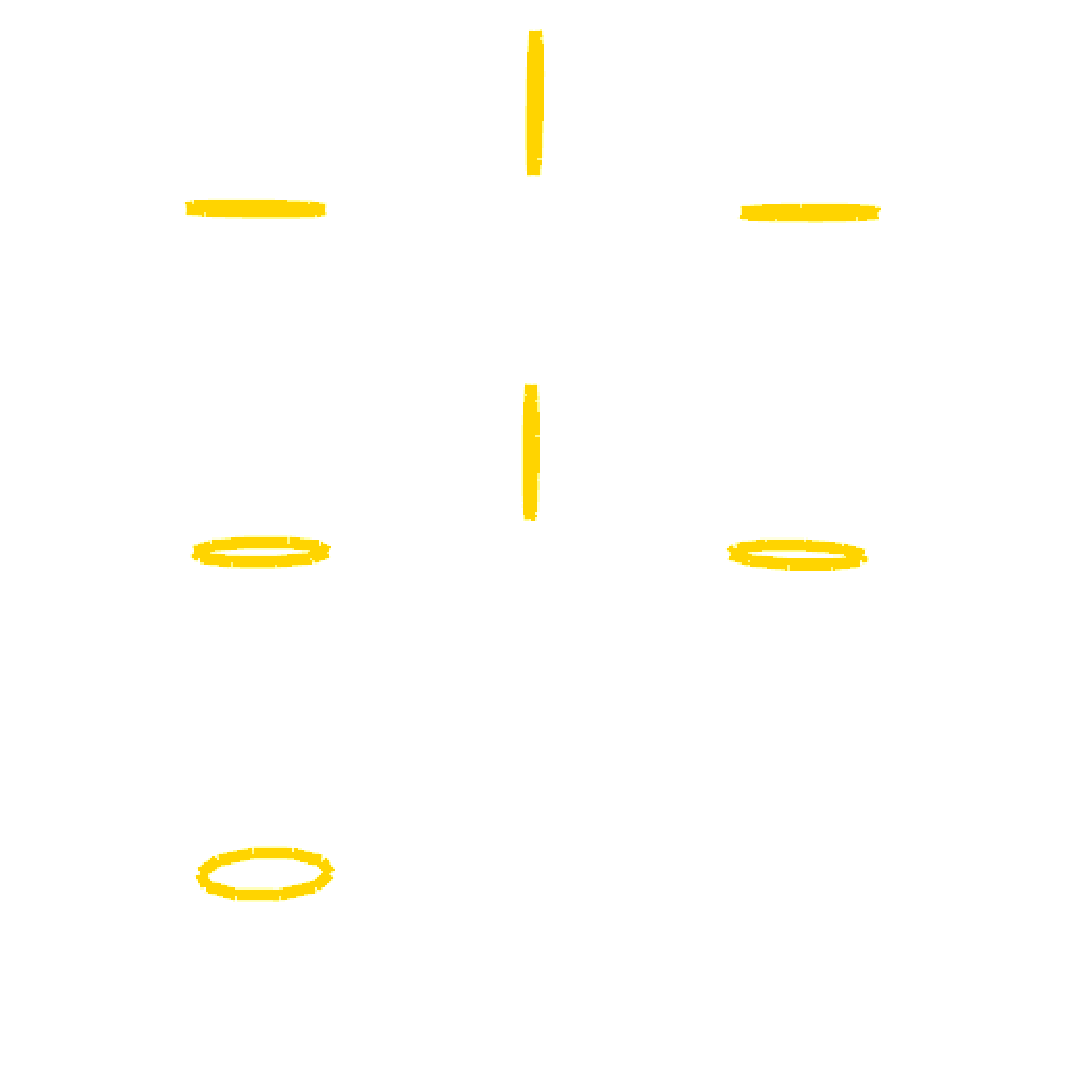
\includegraphics[scale=0.13]{figs/f6.joinFP-input.eps } %0.1
    \end{minipage}}
  \subfigure[]{
    \centering
    \label{fig:fp:b}
    \begin{minipage}[b]{0.18\textwidth}
      \centering
      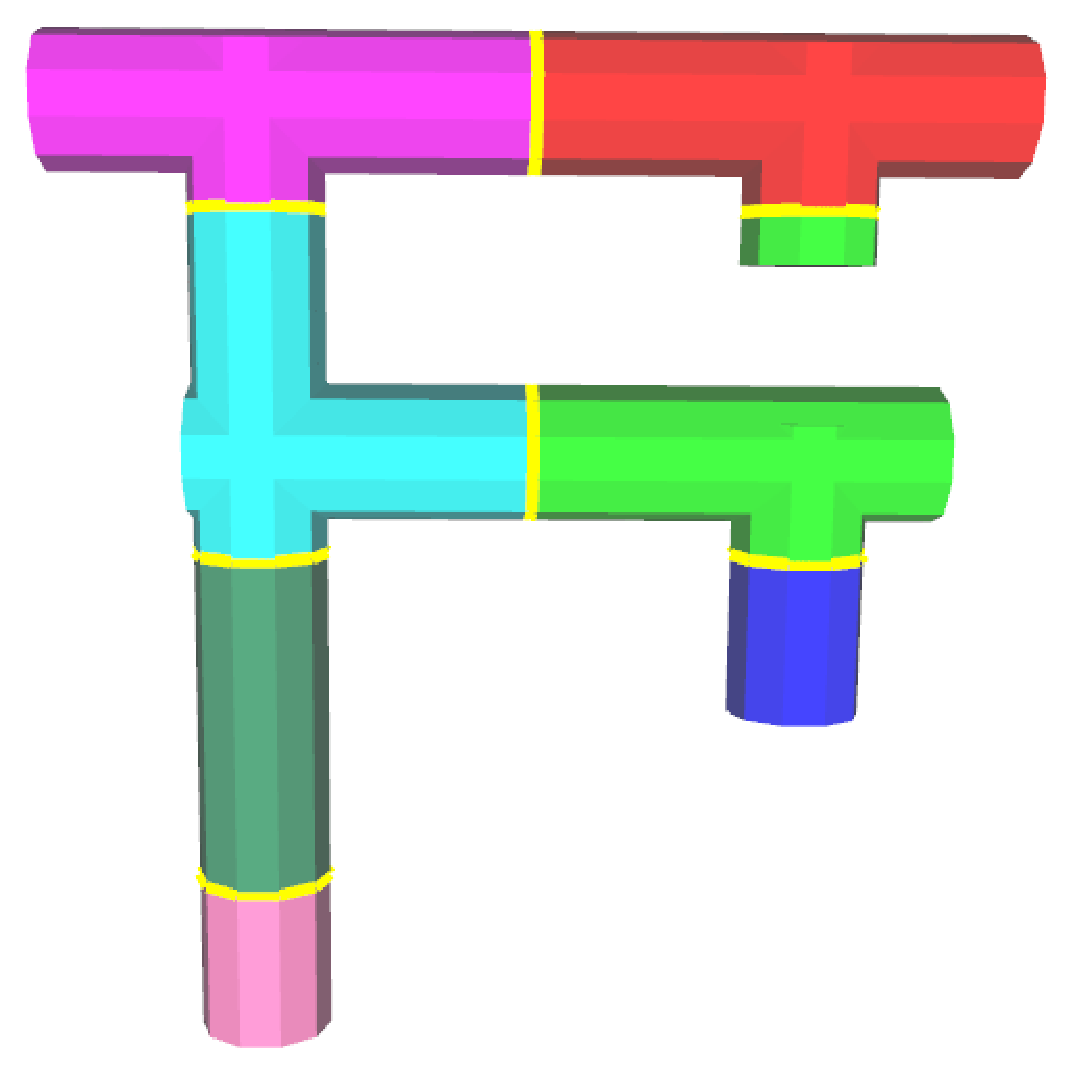
\includegraphics[scale=0.13]{figs/f6.joinFP-F-init.eps}
    \end{minipage}}
  \subfigure[]{
    \label{fig:fp:c}
    \begin{minipage}[b]{0.18\textwidth}
      \centering
      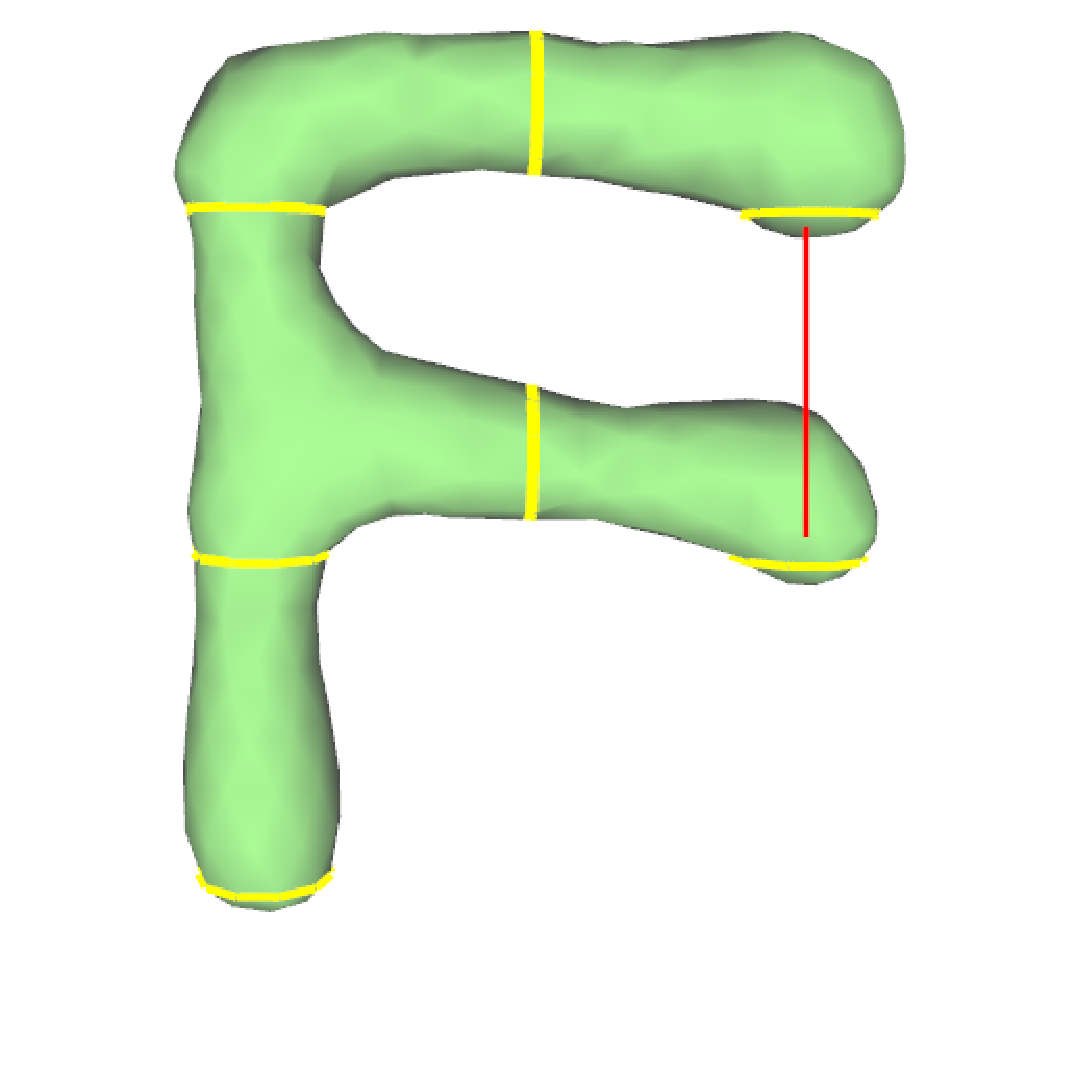
\includegraphics[scale=0.13]{figs/f6.joinFP-join.eps}
    \end{minipage}}
  \subfigure[]{
    \centering
    \label{fig:fp:d}
    \begin{minipage}[b]{0.18\textwidth}
      \centering
      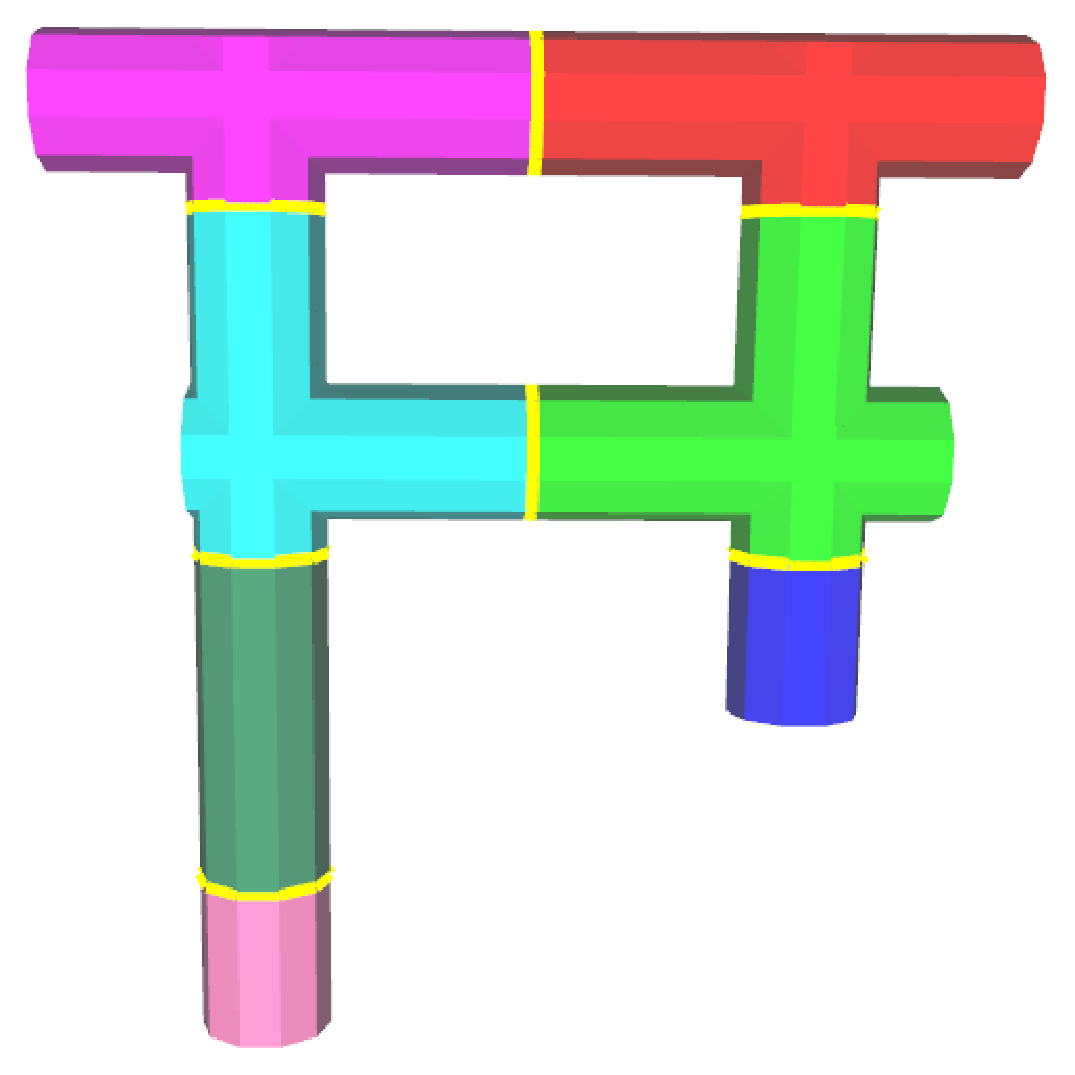
\includegraphics[scale=0.13]{figs/f6.joinFP-P-init.eps}
    \end{minipage}}
  \subfigure[]{
    \centering
    \label{fig:fp:e}
    \begin{minipage}[b]{0.18\textwidth}
      \centering
      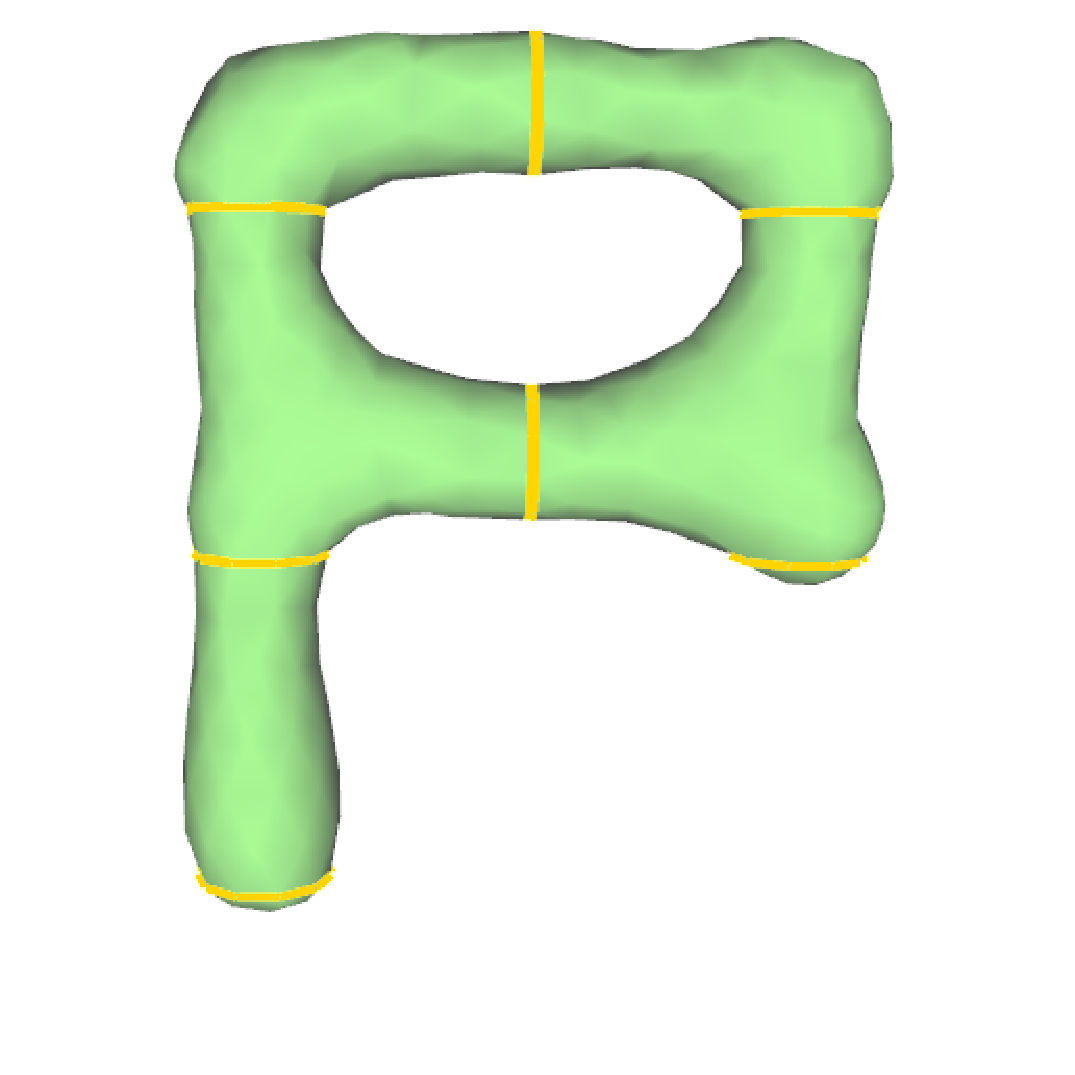
\includegraphics[scale=0.13]{figs/f6.joinFP-P.eps}
    \end{minipage}}
  \caption{An example of the join operation in sketch-based topology editing.
  (a) Input cross sections.
  (b) Computed frusta in zones.
  (c) Sketch a curve (red) on the reconstruction result to join surface parts.
  (d) The corresponding frustum (with light green color) is deformed.
  (e) Editing result.}
  \label{fig:fp}
\end{figure}

In the join operation,  the user is allowed to sketch a curve to
select the two surface parts to be connected (see
Figure~\ref{fig:fp:c}). In the background, the two frusta that are
nearest to the camera among all those selected by the curve will be
selected (the frusta with light green color in
Figure~\ref{fig:fp:b}). If they are in the same zone, then we
compute the centers of the tops of the two selected frusta, and
deform the first selected frustum by moving its top along the vector
pointing from its center to that of the second selected one until
they get intersected (see Figure~\ref{fig:fp:d}). Finally the union
of the frusta within this zone is recomputed and the global surface
is updated (see Figure~\ref{fig:fp:e}). When multiple frusta are
selected in a zone, the last selected one will keep fixed and the
other ones will be deformed in the way to intersect with it.

%illustration on join in two zones
\begin{figure} [htbp]
  \centering
  \subfigure[]{
    \centering
    \label{fig:join2zone:a} %% label for first subfigure
    \begin{minipage}[b]{0.31\textwidth}%\textwidth   %0.31\linewidth
      \centering
      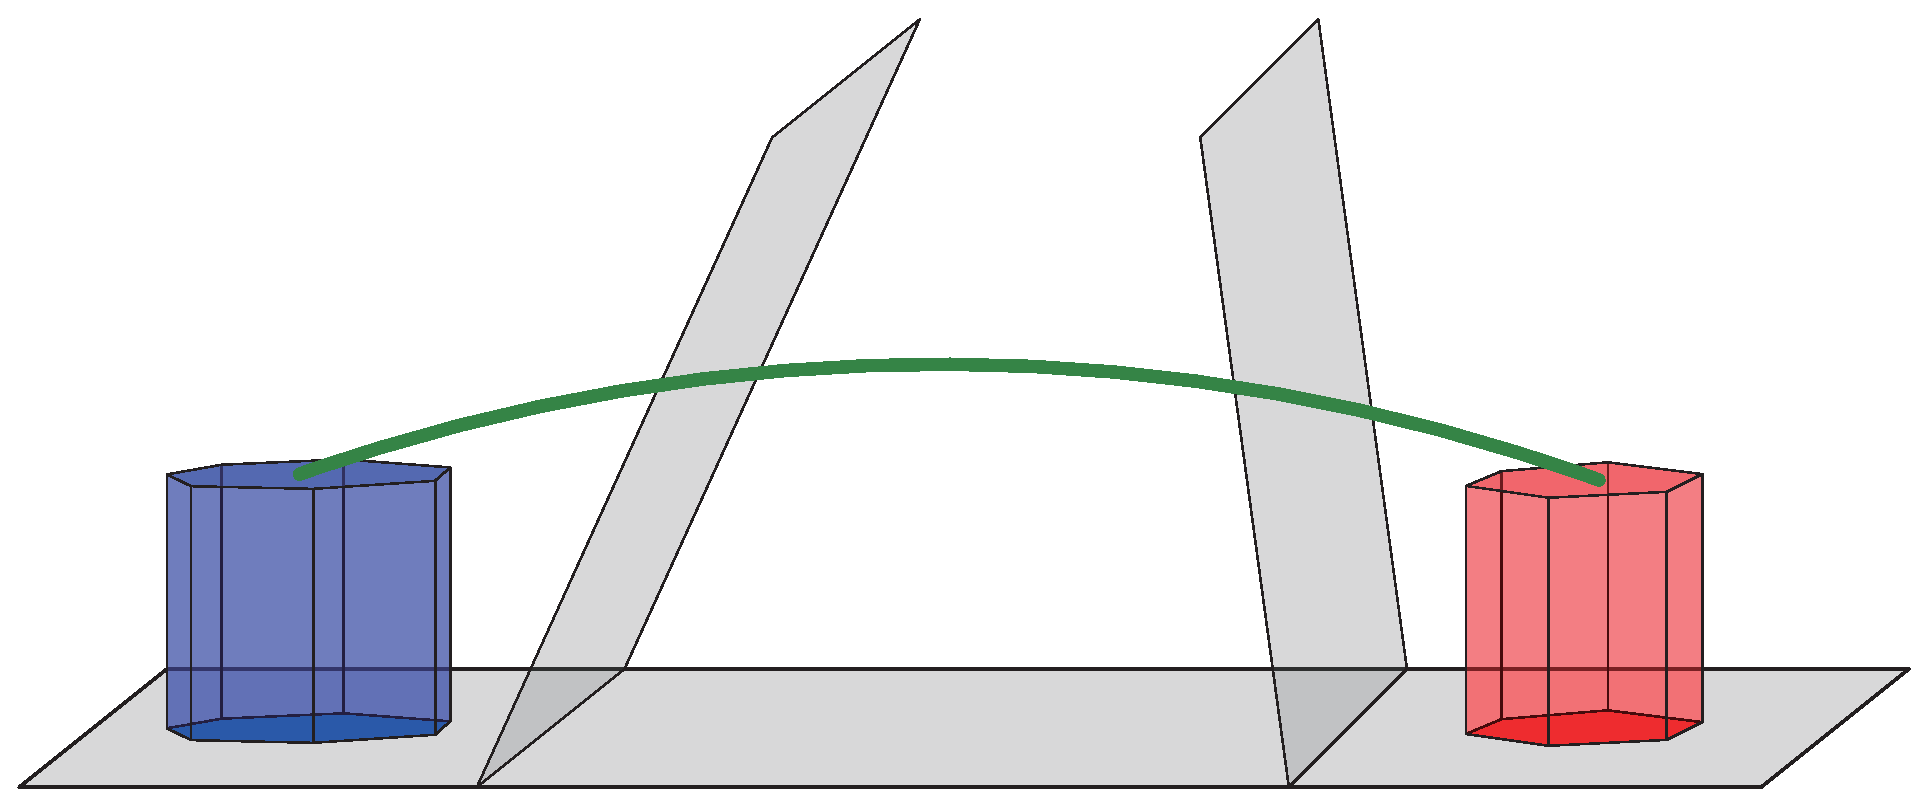
\includegraphics[scale=0.12]{figs/f6.illu-join-2zone-1.eps} %0.08
    \end{minipage}}
  \subfigure[]{
    \centering
    \label{fig:join2zone:b}
    \begin{minipage}[b]{0.31\textwidth}
      \centering
      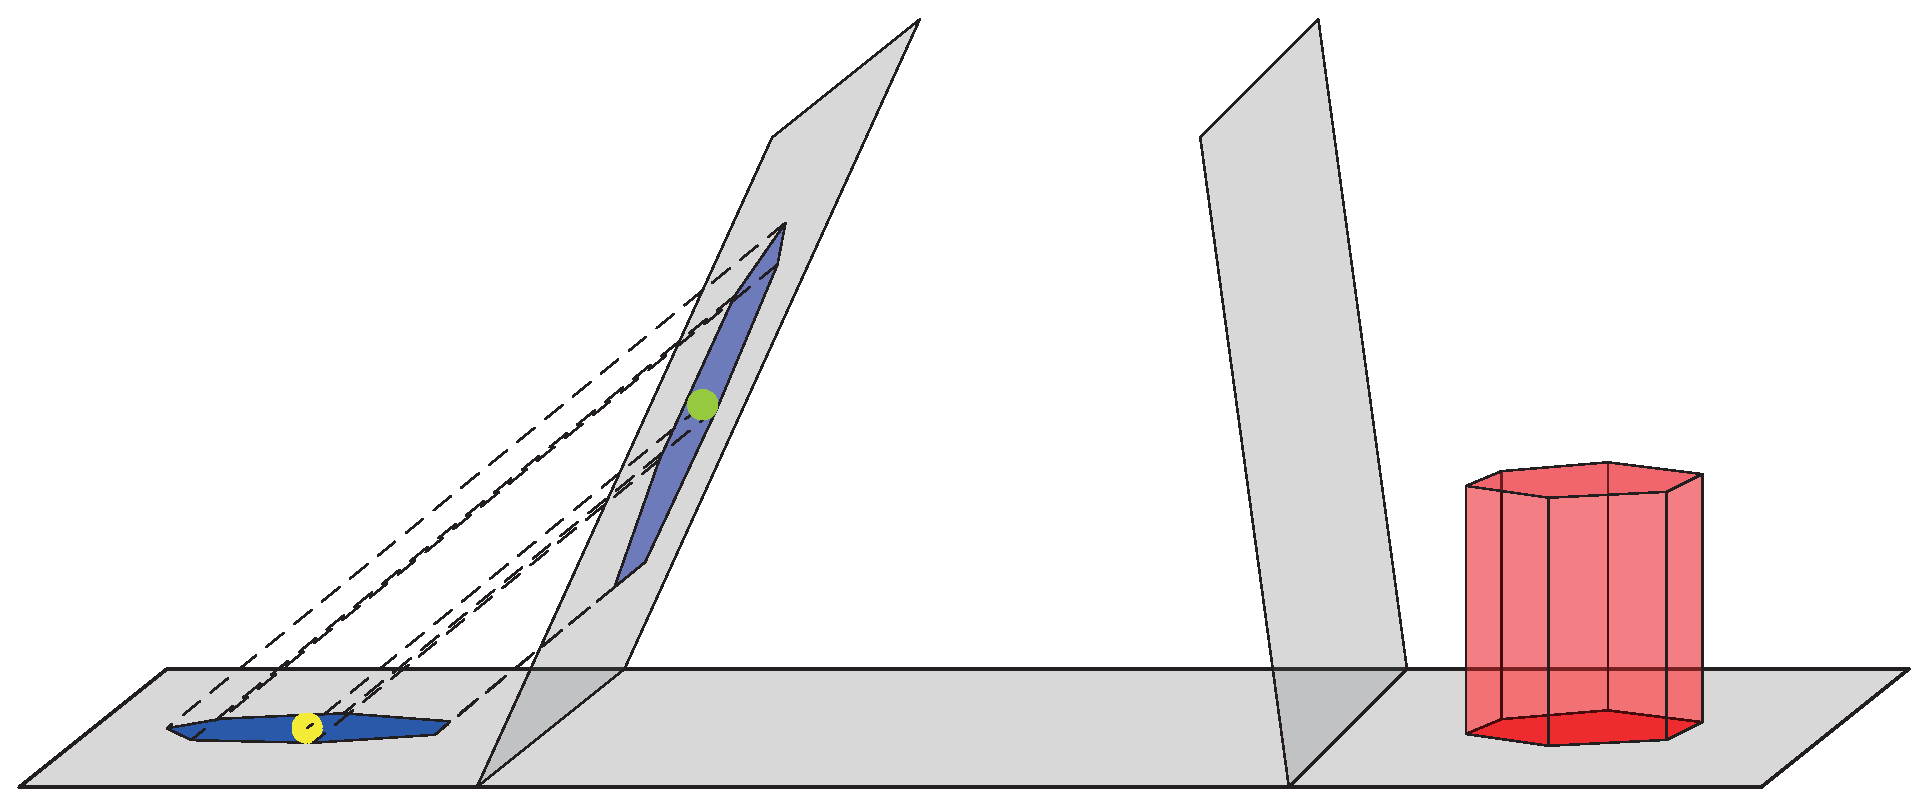
\includegraphics[scale=0.12]{figs/f6.illu-join-2zone-2.eps}
    \end{minipage}}
  \subfigure[]{
    \label{fig:join2zone:c}
    \begin{minipage}[b]{0.31\textwidth}
      \centering
      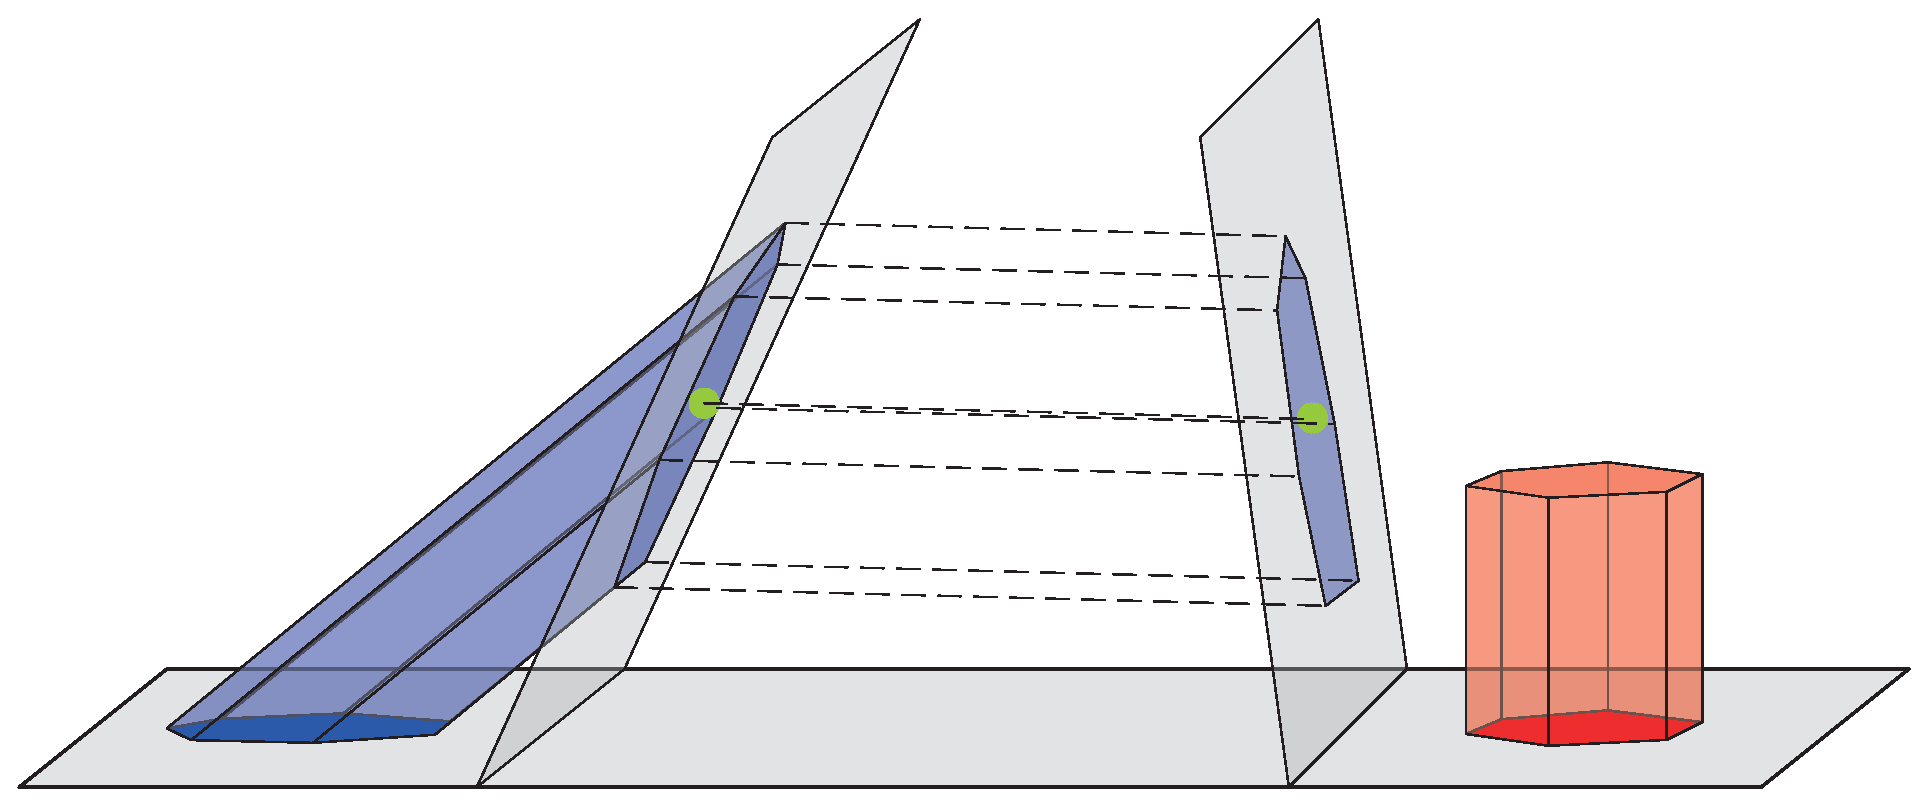
\includegraphics[scale=0.12]{figs/f6.illu-join-2zone-3.eps}
    \end{minipage}}
  \subfigure[]{
    \centering
    \label{fig:join2zone:d}
    \begin{minipage}[b]{0.31\textwidth}
      \centering
      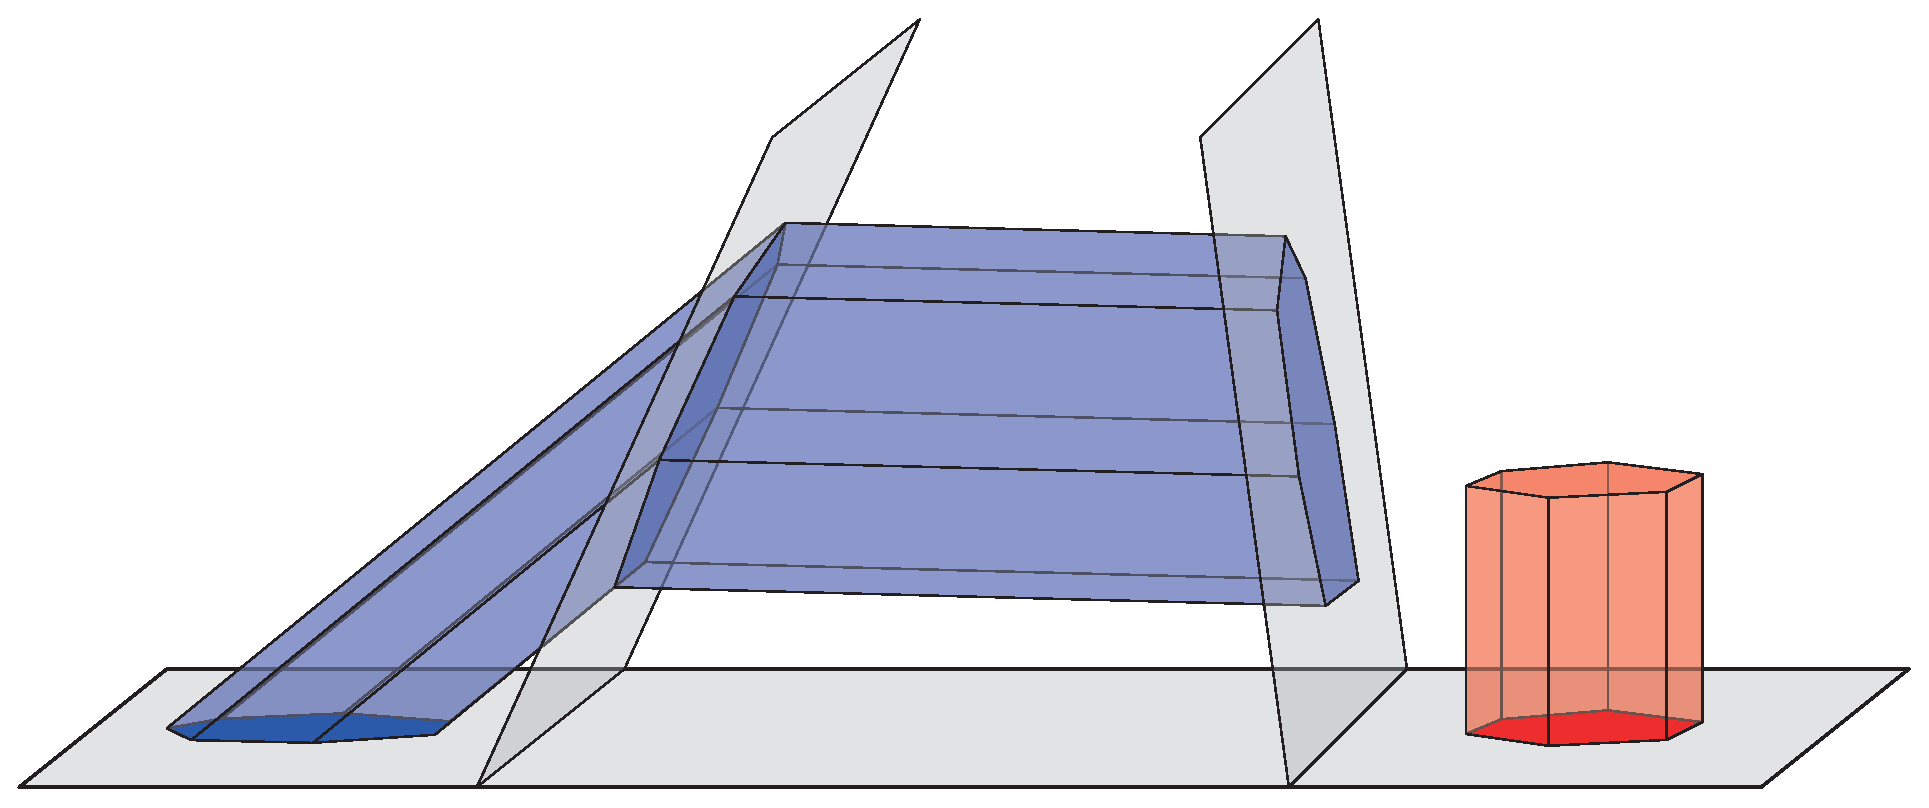
\includegraphics[scale=0.12]{figs/f6.illu-join-2zone-4.eps}
    \end{minipage}}
  \subfigure[]{
    \centering
    \label{fig:join2zone:e}
    \begin{minipage}[b]{0.31\textwidth}
      \centering
      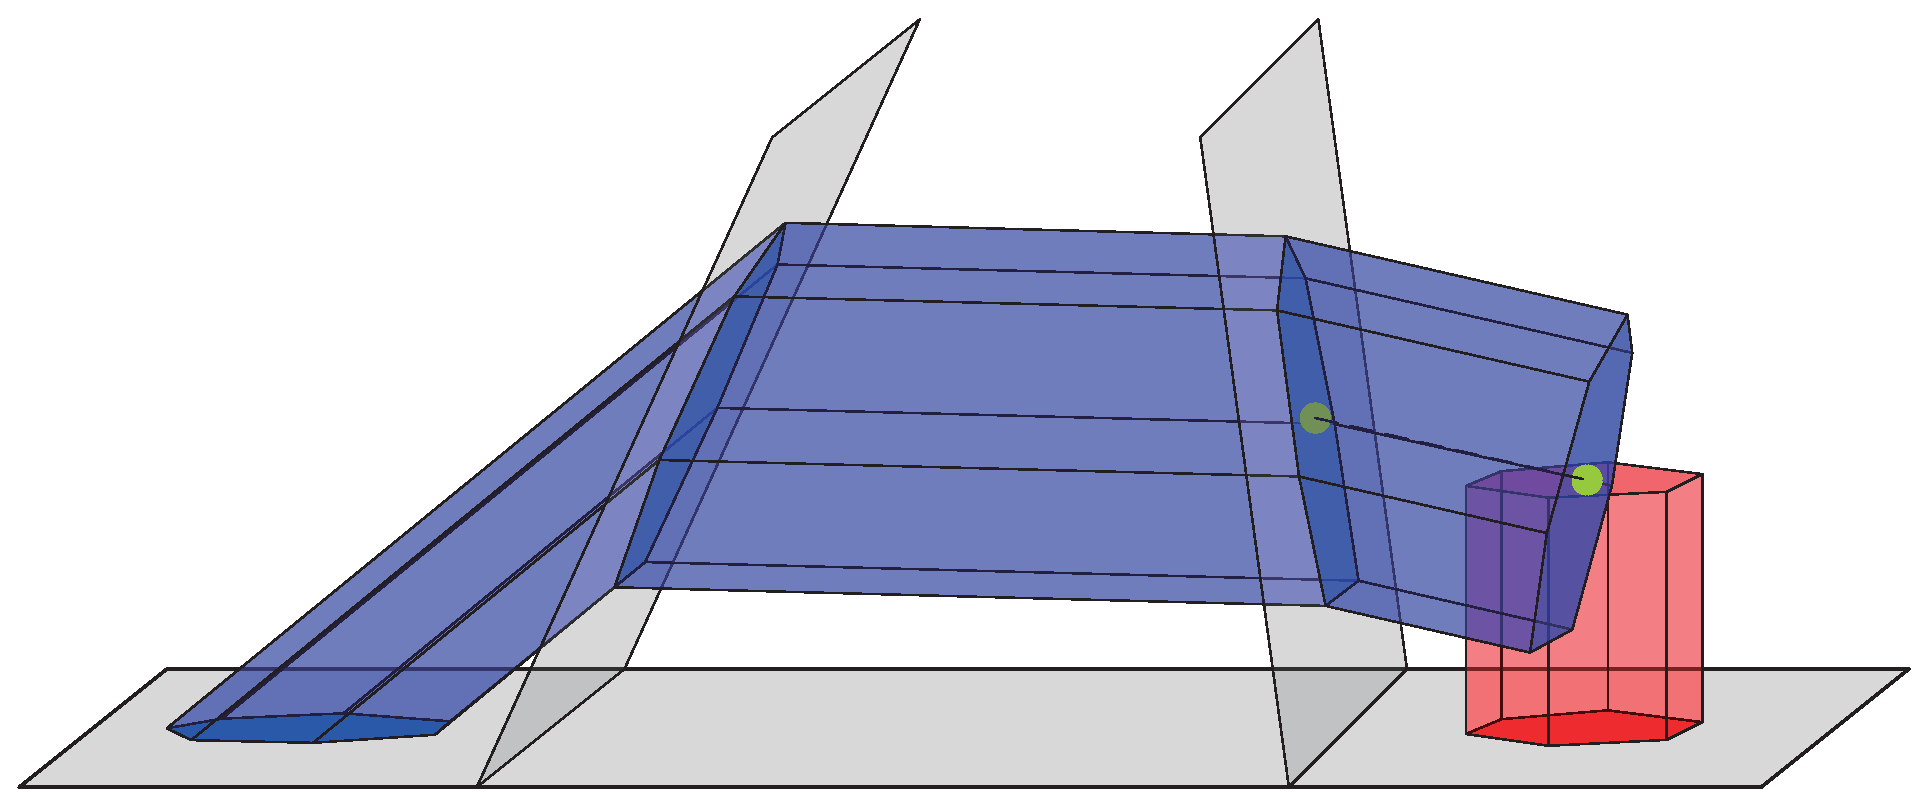
\includegraphics[scale=0.12]{figs/f6.illu-join-2zone-5.eps}
    \end{minipage}}
  \subfigure[]{
    \centering
    \label{fig:join2zone:f}
    \begin{minipage}[b]{0.31\textwidth}
      \centering
      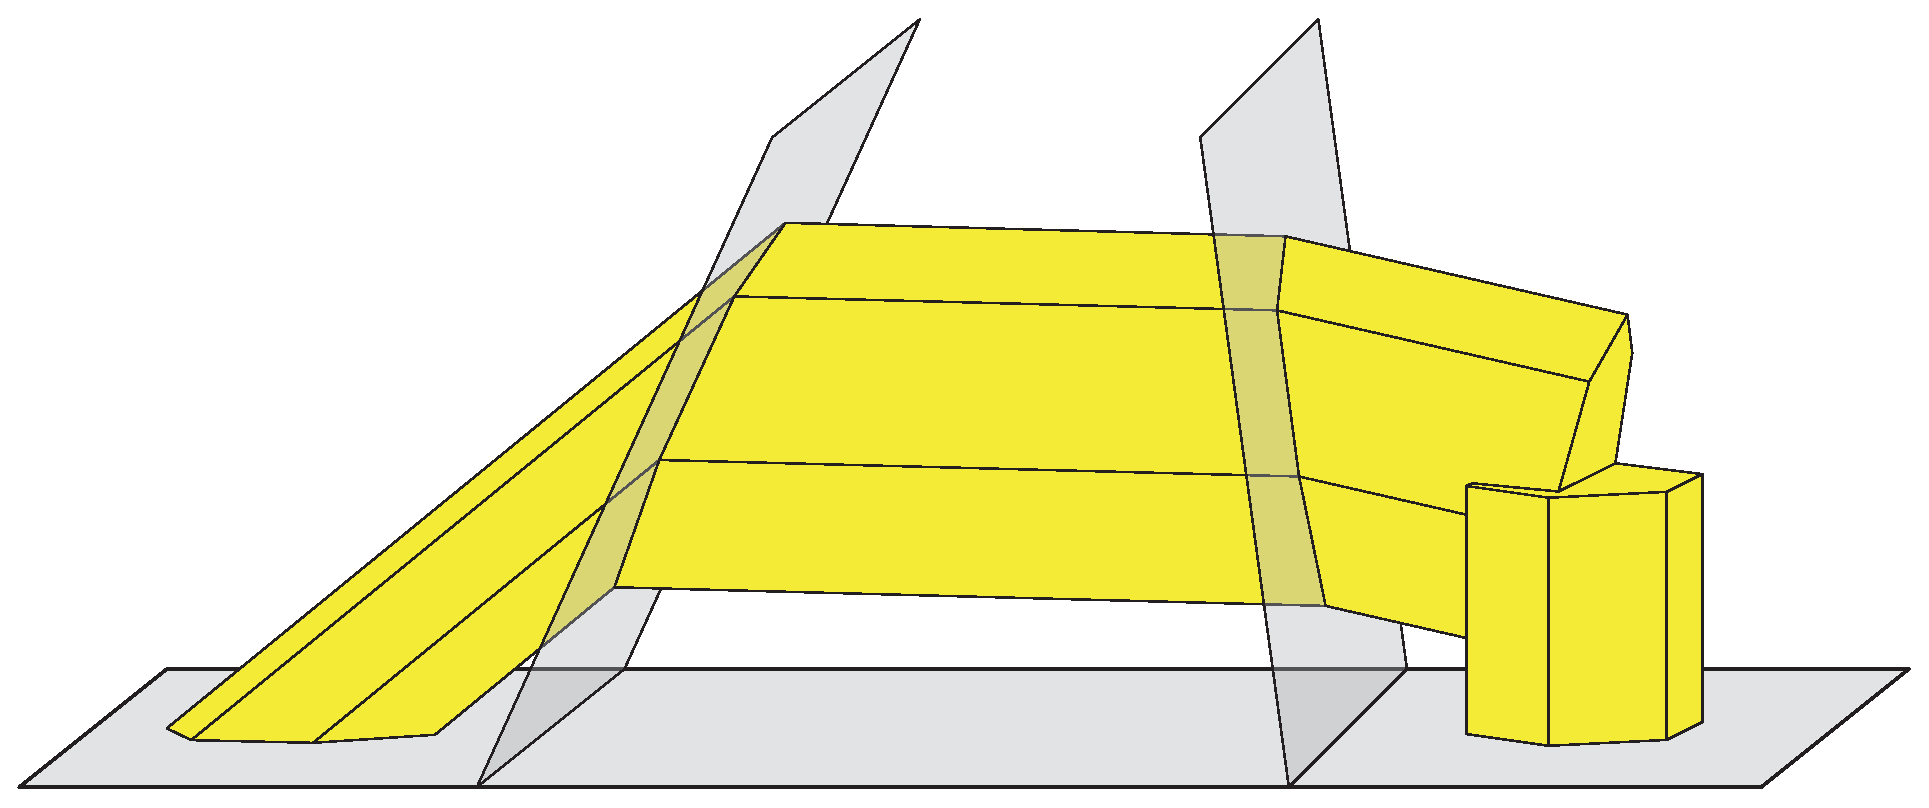
\includegraphics[scale=0.12]{figs/f6.illu-join-2zone-6.eps}
    \end{minipage}}
  \caption{Illustration of the join of surface parts in different zones.
  (a) Sketch a curve (green) to select the two frusta.
  (b) Re-calculate the top of the first selected frustum by projecting its bottom onto the common face with the neighbor zone.
  (c)-(d) Extend the frustum.
  (e) Build the extended frustum in the zone containing the second selected frustum.
  (f) Editing result.}
  \label{fig:join2zone}
\end{figure}

We also allow  the join of surface parts in different zones. In that
case, the two frusta and the zones they belong to will be firstly
selected (see Figure~\ref{fig:join2zone:a}). Then we need to find a
series of adjacent zones connecting these two zones. To do that, we
start this searching process from the first selected zone, to find
its neighboring zones whose 2D projections on the screen contain the
points of the sketched 2D curve. This searching process continues
from these candidate zones until the last selected zone is reached.
A set of zones connecting the first and last selected zones, as well
as the common faces incident to each pair of zones can thus be
obtained. Next, we re-calculate the first selected frustum by
projecting its bottom onto the first calculated common face to get
the new top (see Figure~\ref{fig:join2zone:b}) and continue
extending the frustum across the selected zones in this way until
the last zone is reached (see Figure~\ref{fig:join2zone:c}
and~\ref{fig:join2zone:d}). Note that this method is quite similar
to that we used in Section~\ref{ch6:sec:reconst:end}. However, since
the dihedral angle between the plane of the face $f_t$ to project
and that of the face $f_b$ containing the bottom of the frustum may
not be acute, projecting in the orthogonal direction of $f_t$ will
not work in that case. So here we project the bottom of each frustum
along the direction pointing from its center to that of $f_t$, to
get the frustum top. The top of the extended frustum in the last
zone will be calculated by translating the bottom along the vector
pointing from its center to that of the top of the second selected
frustum (see Figure~\ref{fig:join2zone:e}) such that the two frustum
can get intersected (see Figure~\ref{fig:join2zone:f}).





\subsection{The split operation}
\label{ch6:sec:edit:split}

%B->E example
\begin{figure} [htbp]
  \centering
  \subfigure[]{
    \centering
    \label{fig:be:a} %% label for first subfigure
    \begin{minipage}[b]{0.22\textwidth} %linewidth
      \centering
      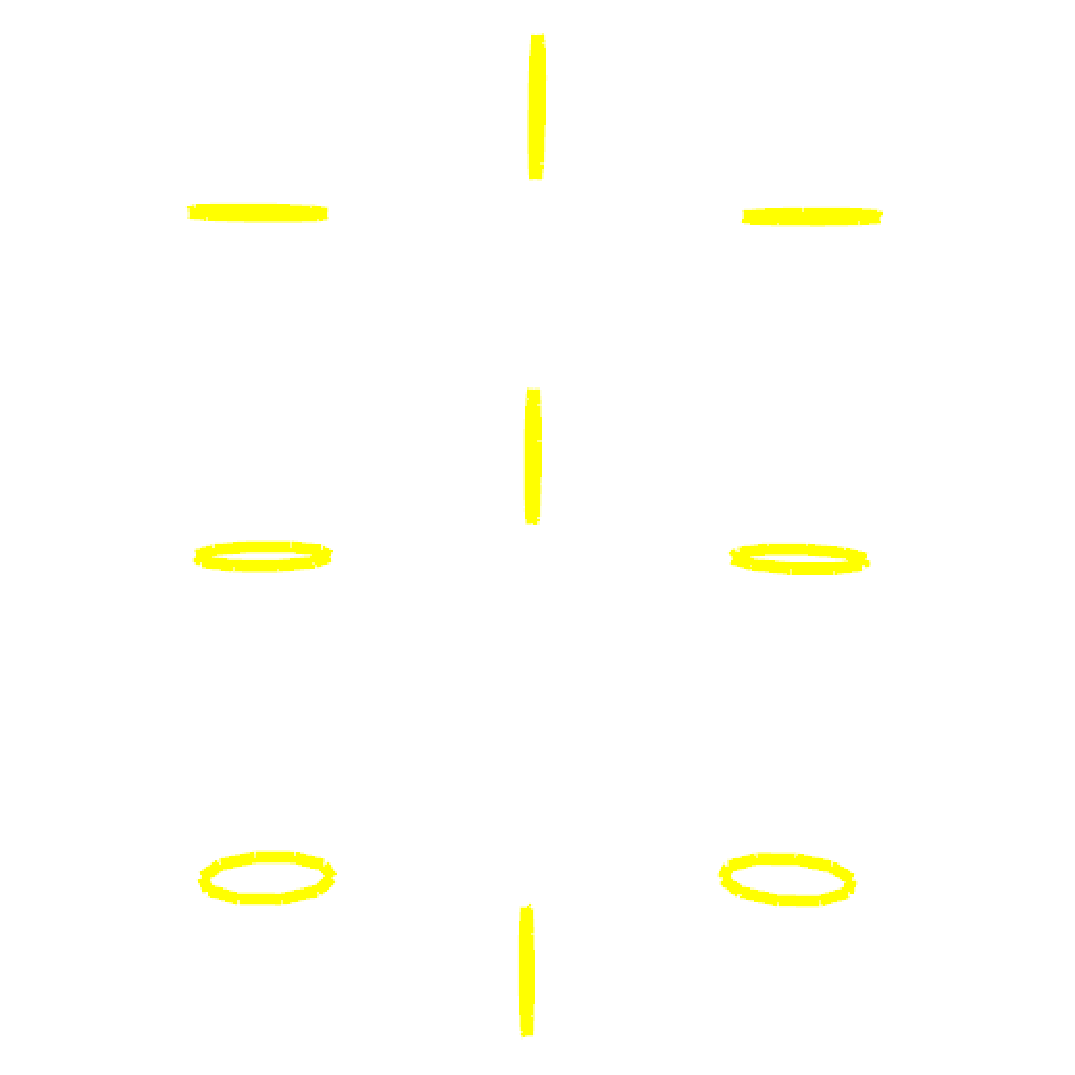
\includegraphics[scale=0.13]{figs/f6.BEsplit-input.eps} %0.1
    \end{minipage}}
  \subfigure[]{
    \centering
    \label{fig:be:b}
    \begin{minipage}[b]{0.22\textwidth}
      \centering
      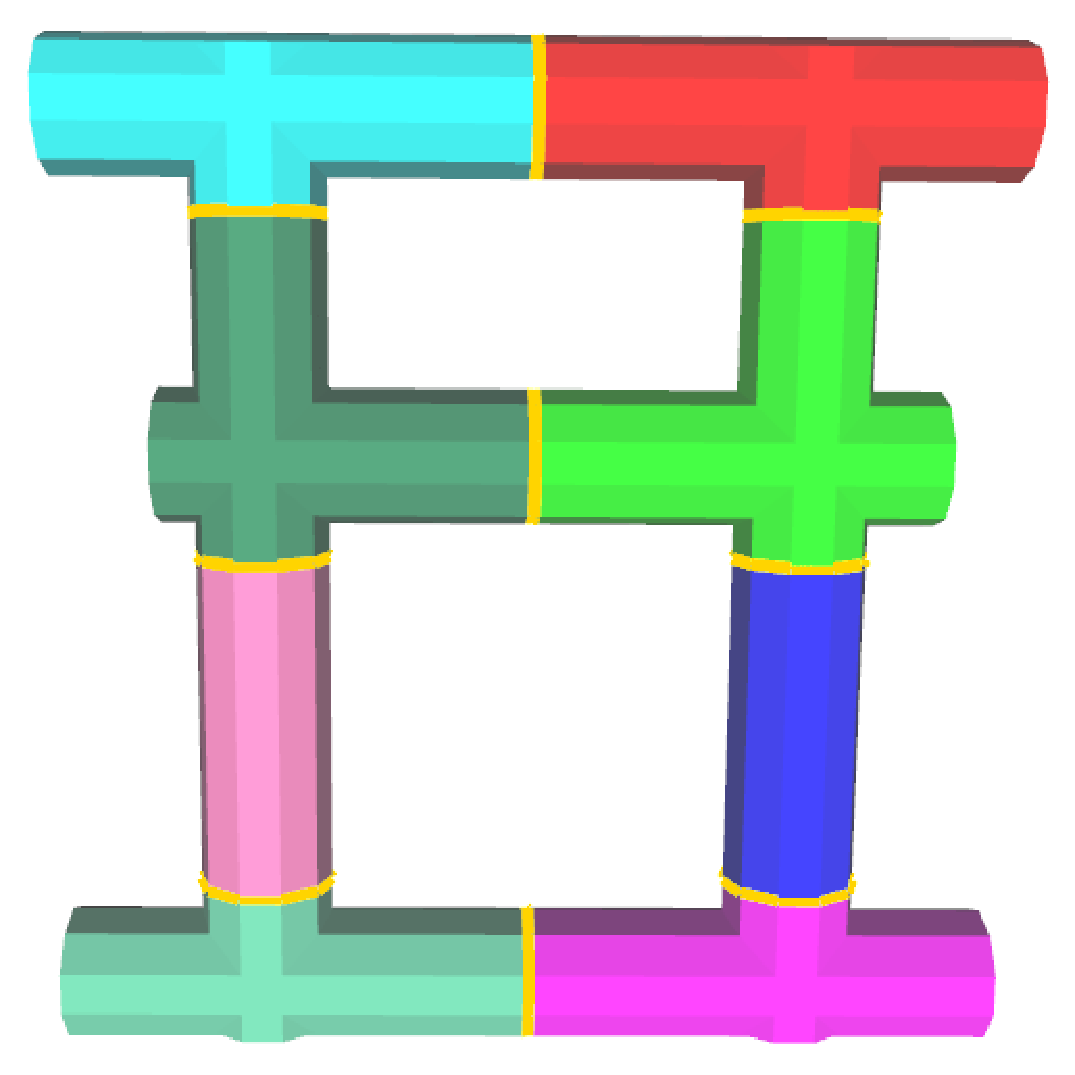
\includegraphics[scale=0.13]{figs/f6.BEsplit-B-init.eps}
    \end{minipage}}
  \subfigure[]{
    \label{fig:be:c}
    \begin{minipage}[b]{0.22\textwidth}
      \centering
      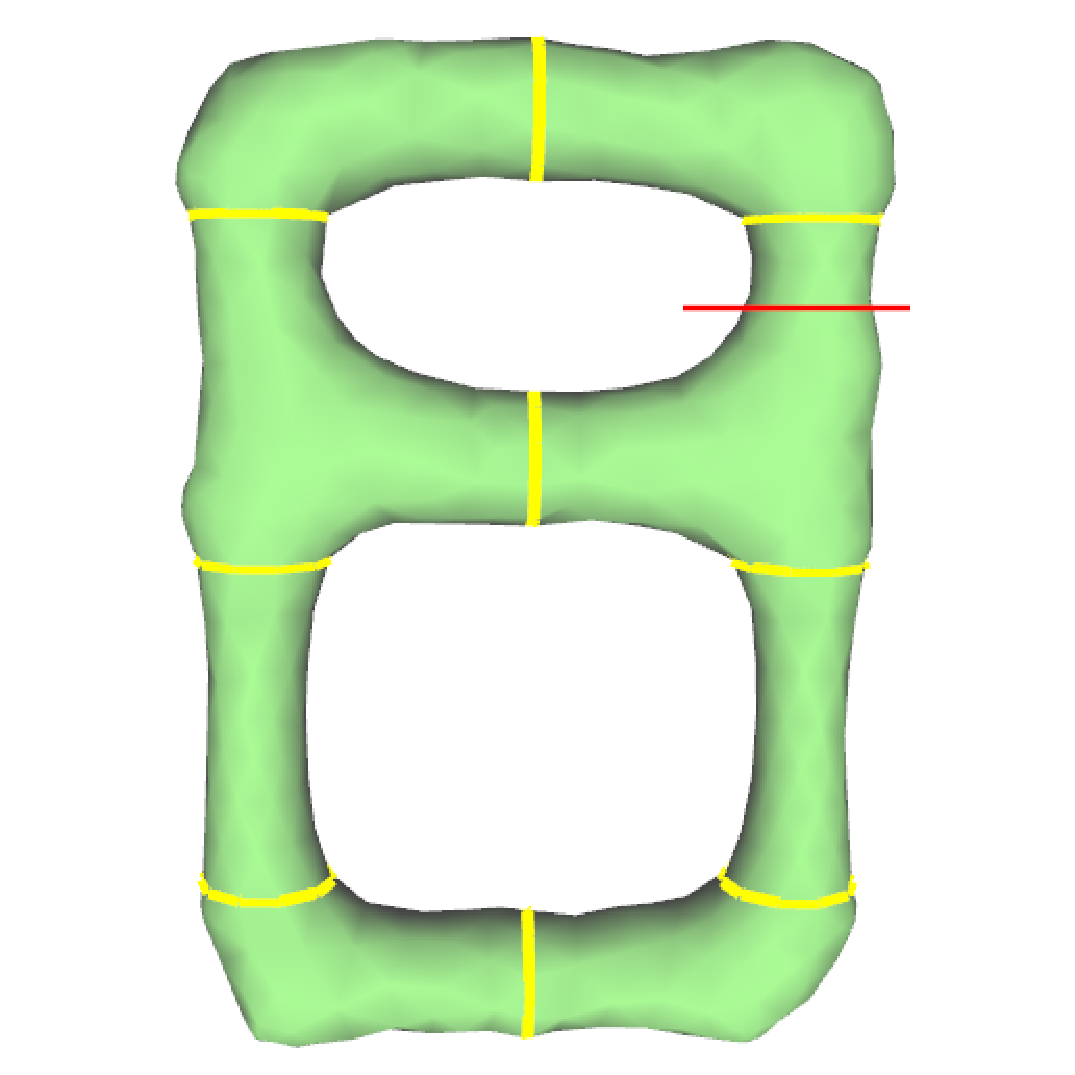
\includegraphics[scale=0.13]{figs/f6.BEsplit-split1.eps}
    \end{minipage}}
  \subfigure[]{
    \centering
    \label{fig:be:d}
    \begin{minipage}[b]{0.22\textwidth}
      \centering
      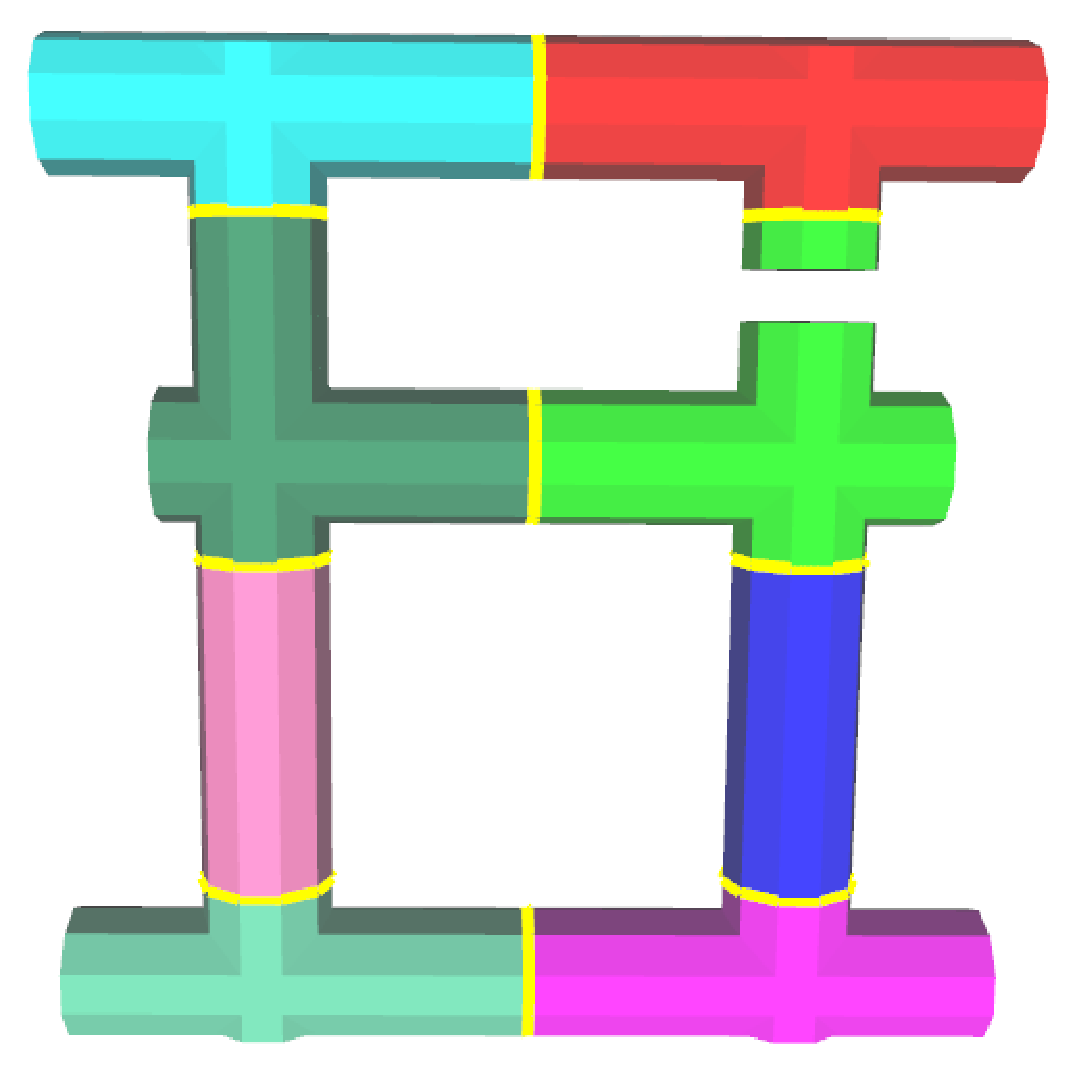
\includegraphics[scale=0.13]{figs/f6.BEsplit-inbetween-init.eps}
    \end{minipage}}
  \\
  \subfigure[]{
    \centering
    \label{fig:be:e}
    \begin{minipage}[b]{0.22\textwidth}
      \centering
      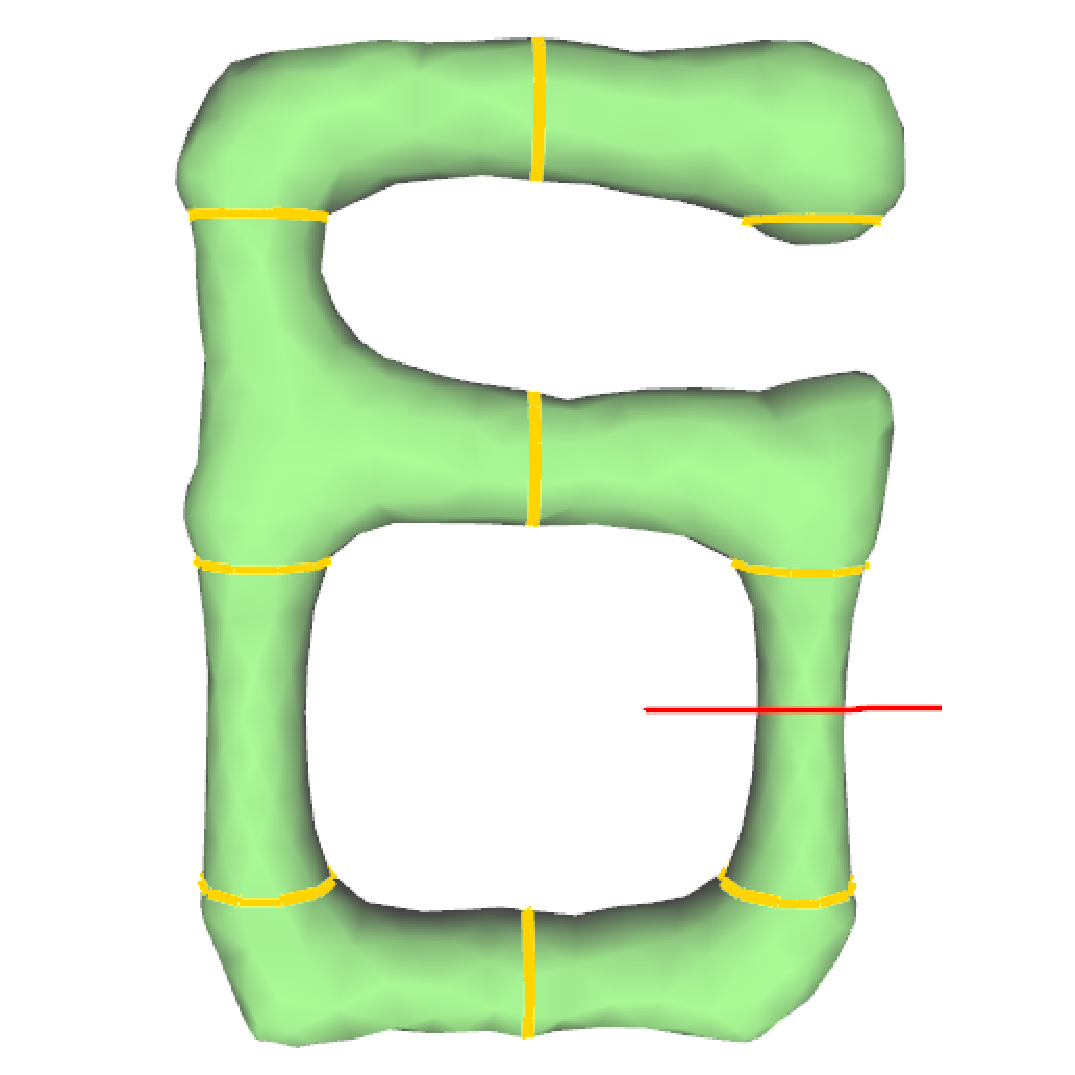
\includegraphics[scale=0.13]{figs/f6.BEsplit-split2.eps}
    \end{minipage}}
  \subfigure[]{
    \centering
    \label{fig:be:f}
    \begin{minipage}[b]{0.22\textwidth}
      \centering
      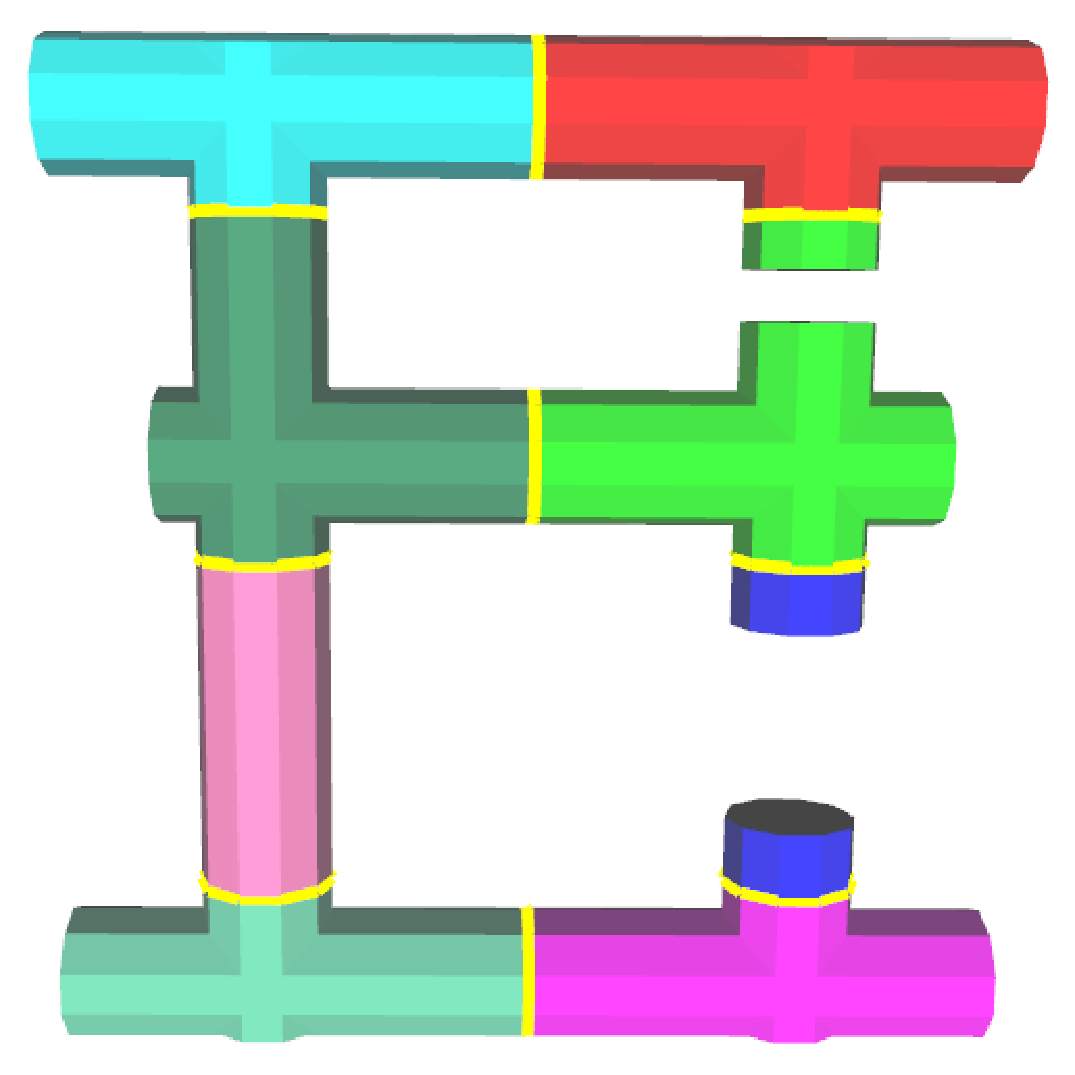
\includegraphics[scale=0.13]{figs/f6.BEsplit-E-init.eps}
    \end{minipage}}
  \subfigure[]{
    \centering
    \label{fig:be:g}
    \begin{minipage}[b]{0.22\textwidth}
      \centering
      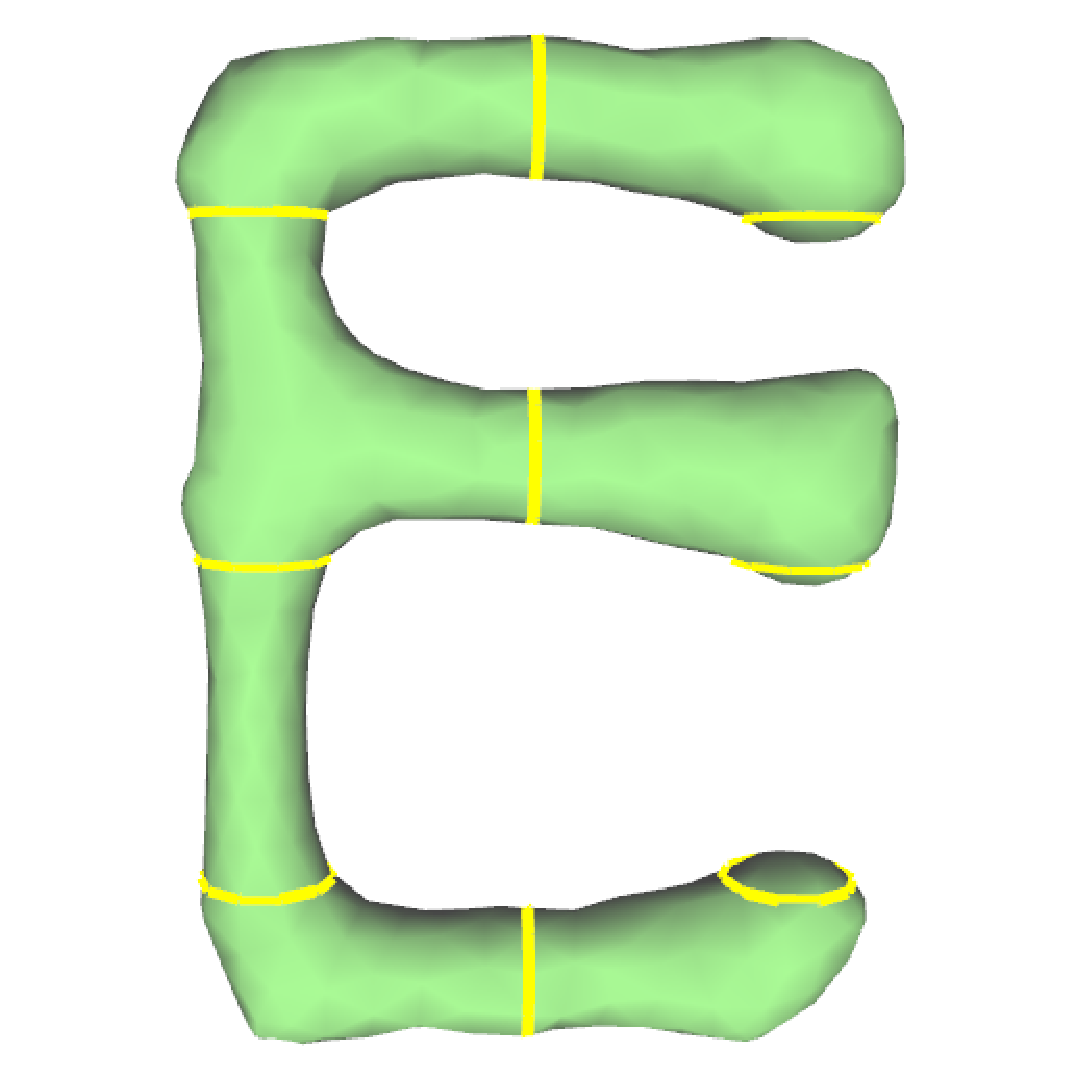
\includegraphics[scale=0.13]{figs/f6.BEsplit-E.eps}
    \end{minipage}}
  \caption{An example of the split operation in sketch-based topology editing.
  (a) Input cross sections.
  (b) Computed frusta in zones.
  (c) Sketch a curve (red) on the reconstruction result to split local surface.
  (d) The corresponding frusta (with light green color) are shrunk to be separated.
  (e) Sketch another split curve on the updated model.
  (f) The corresponding blue frusta are shrunk.
  (g) Editing result.}
  \label{fig:be}
\end{figure}

The split operation applies  to the local components that are formed
from connected surface parts generated from two or more cross
sections within the same zone. If the component to split is
generated from one single cross section in a zone, splitting it will
produce an extra isolated surface component which does not
interpolate any cross section curves in this zone. To split a local
surface component, the user needs to first adjust the viewpoint to
make it foremost and then sketch a cutting curve passing through
it(see Figure~\ref{fig:be:c} and~\ref{fig:be:e}). Next all the
connected frusta that contribute to the selected surface part are
selected and shrunk towards their bottoms until they do not
intersect (The light green frusta in Figure~\ref{fig:be:d} and the
blue frusta in Figure~\ref{fig:be:f}). This guarantees that the
surface parts obtained after the union operation will be separated.
The global surface can then be updated.


%significancy
It can be seen that  by making use of the generated frusta obtained
in the reconstruction process in the local topology editing
operations, our approach builds a bridge that efficiently connects
the two originally independent operations, such that a desired shape
can be produced for the user through simple sketches and local
computation when the initial reconstruction result is not
satisfactory. The final surface produced by our surface
reconstruction framework will have regular local shapes and be
composed of only one component.

It should be mentioned  that the two editing operations can also be
incorporated into the surface reconstruction step, by adopting
strategies to set the shape of the generated frusta. For example, we
can force each frustum to be connected with others, such that the
output surface after the first reconstruction step will be
guaranteed to have a single component. However, this compulsive
integration may produce irregular local shapes and unexpected
connectivity of different surface parts. Thus we just try to produce
a valid model with regular shapes in the first step and leave the
adjustment of the local topology to the user.




%%%%%%%%%%%%%%%%%%%%%%%%%%%%%%%%%%%%%%%%%%%%%%%%%%%%%%%%%%%%%%%%%%%%%%%%%%%%%%%%%%%
%%---------------------------------------------------------------------------------
\section{Results and discussions}
\label{ch6:sec:result}

%reconstruction examples:cactus, hand, stomach, teacup, tooth, tree
\begin{figure*} [htbp]
  \centering
  \subfigure[The \textit{Cactus} model]{
    \centering
    \label{fig:eg:a} %% label for first subfigure
    \begin{minipage}[b]{0.48\textwidth}%0.48
      \centering
      \includegraphics[scale=0.09]{figs/f6.cactus.eps}%0.1
    \end{minipage}}
  \subfigure[The \textit{Teacup} model]{
    \centering
    \label{fig:eg:b}
    \begin{minipage}[b]{0.48\textwidth}%0.48
      \centering
      \includegraphics[scale=0.07]{figs/f6.teacup.eps}%0.08
    \end{minipage}}
  \subfigure[The \textit{Tooth} model]{
    \label{fig:eg:c}
    \begin{minipage}[b]{0.45\textwidth}%0.46
      \centering
      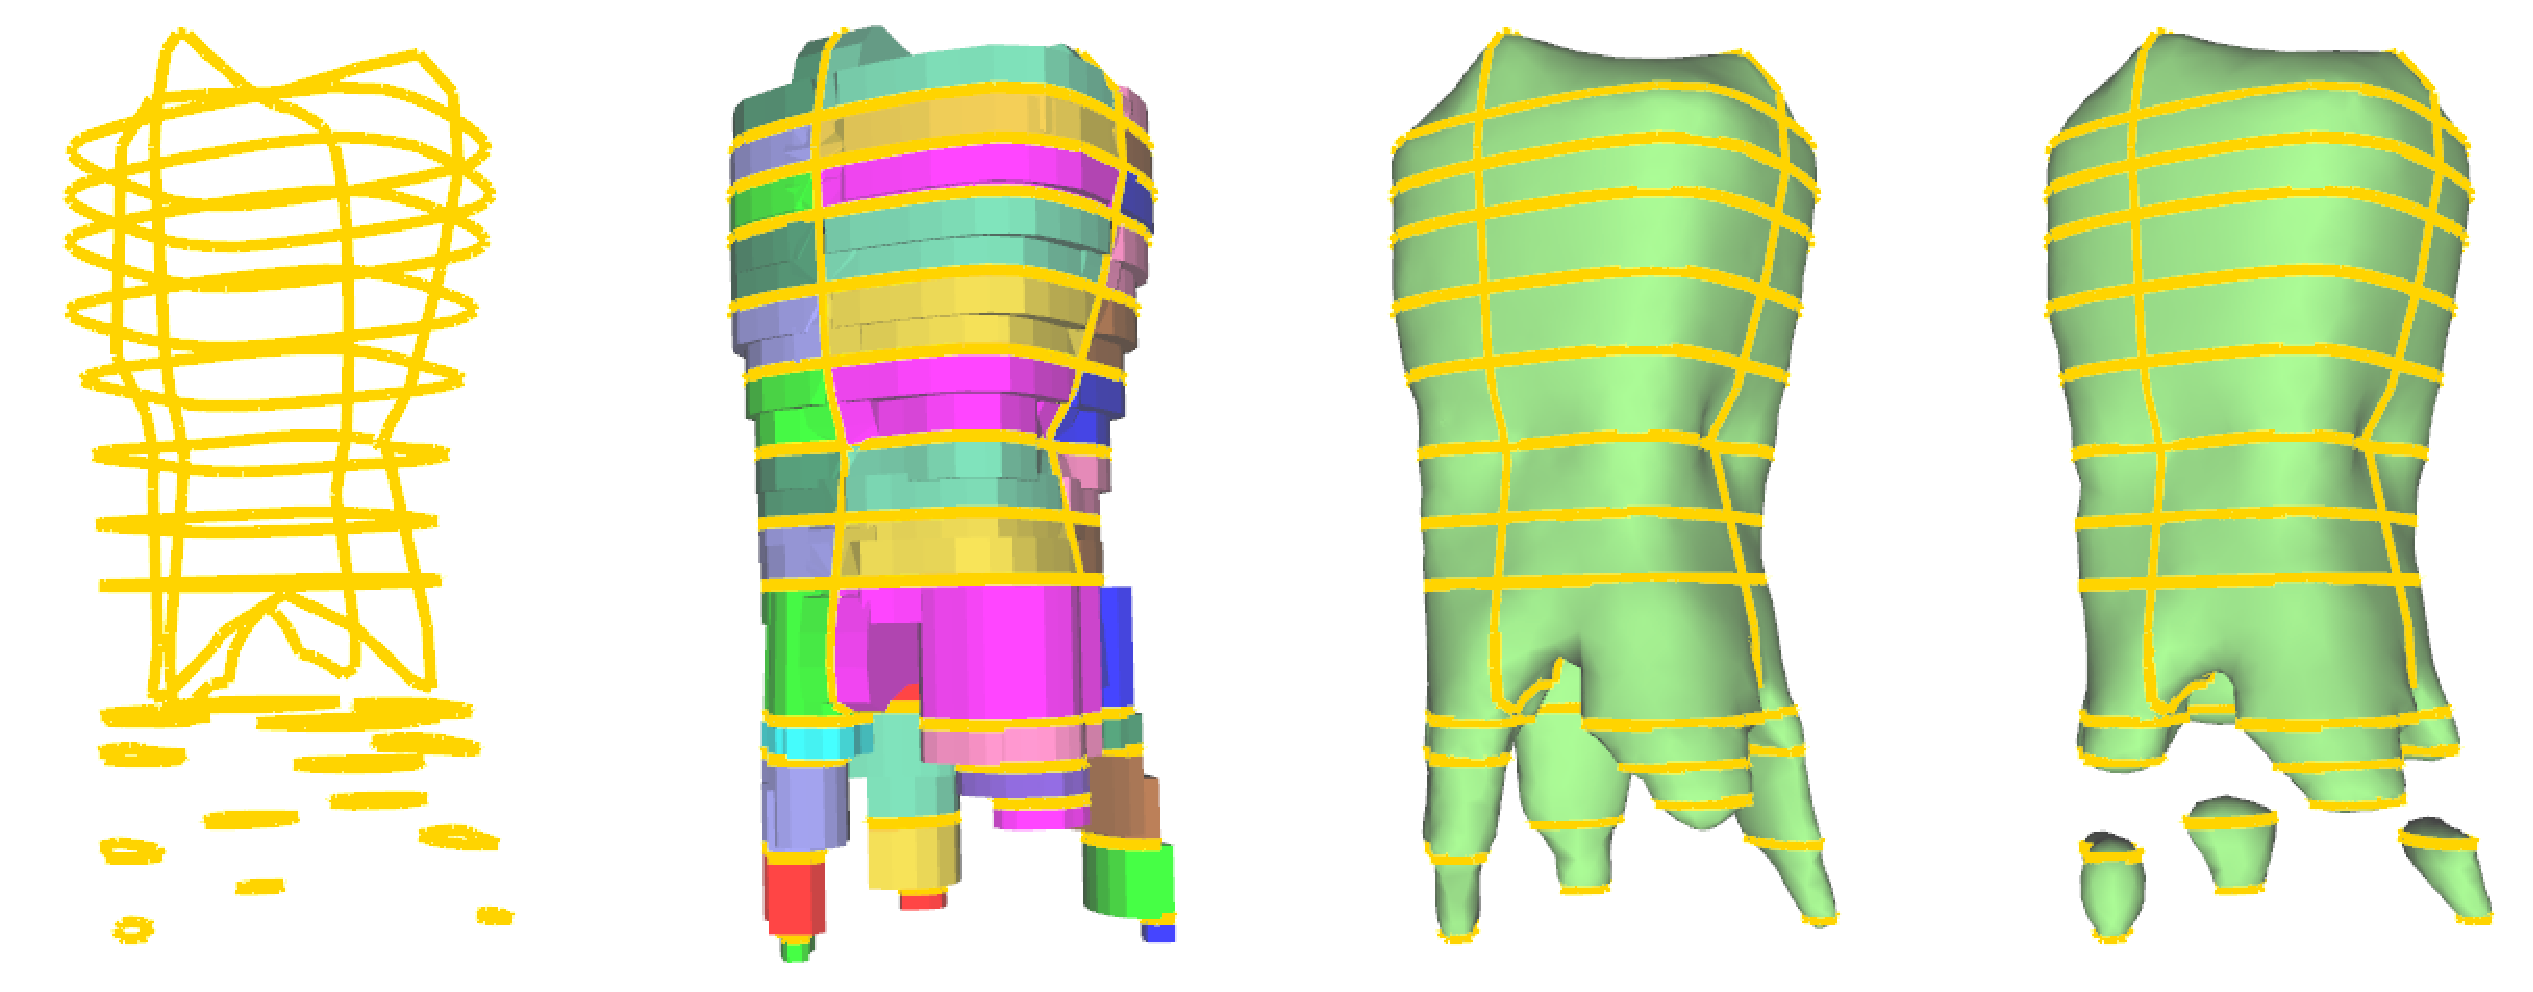
\includegraphics[scale=0.13]{figs/f6.tooth.eps}%0.14
    \end{minipage}}
  \subfigure[The \textit{Tree} model]{
    \label{fig:eg:d}
    \begin{minipage}[b]{0.51\textwidth}%0.52
      \centering
      \includegraphics[scale=0.08]{figs/f6.tree.eps}%0.09
    \end{minipage}}
  \subfigure[The \textit{Stomach} model]{
    \centering
    \label{fig:eg:f}
    \begin{minipage}[b]{0.45\textwidth}%0.46
      \centering
      \includegraphics[scale=0.09]{figs/f6.stomach.eps}%0.1
    \end{minipage}}
  \subfigure[The \textit{Hand} model]{
    \centering
    \label{fig:eg:e}
    \begin{minipage}[b]{0.51\textwidth}%0.52
      \centering
      \includegraphics[scale=0.11]{figs/f6.hand.eps}%0.12
    \end{minipage}}
  \caption{Results of our surface reconstruction algorithm. In each example, the input cross sections, the generated sub-surfaces in zones, the reconstruction result of our algorithm, and the result of the algorithm of~\cite{LBDLJ08} are shown in order.}
  \label{fig:eg}
\end{figure*}


%implementation details
We have demonstrated our surface reconstruction algorithm on both
the bio-medical and synthetic models in Figure~\ref{fig:eg}. Cross
sections on arbitrary planes with complex relationship were taken as
the input to test the universality and robustness of the algorithm.
These cross sections are computed from the models provided in the
INRIA Gamma team research database~\cite{INRIA}. For comparison, we also present
the results generated using the algorithm of~\cite{LBDLJ08}, which
represents the state-of-the-art and is closely related to our work.

By extending the surface  components generated in the \textit{end}
zones and adjusting the shape of the generated frusta to connect
isolated surface parts, our algorithm can produce a manifold surface
with only one connected component. All the examples in
Figure~\ref{fig:eg} have demonstrated this advantage of our scheme
over the existing methods which use the traditional partition
approach. This is more obvious on the shapes with multiple branches
than those with topology equivalent to a simple sphere. This is
because in the former case, the distribution and relationship of
cross sections are more complicated and faces which may separate the
connections of different surface components are more likely to
exist.

Since our sub-surface reconstruction  is independent of any
geometric agency (eg, the medial axis plane in~\cite{LBDLJ08}),
topological noise caused by the irregularity of the agency in
previous methods can be eliminated. Such an example can be seen in
Figure~\ref{fig:eg:e}, in which undesired artifacts are created in
the local surface between the thumb and palm in the result
of~\cite{LBDLJ08} but are avoided in our result.

%editing examples:skull
\begin{figure*} [htbp]
  \centering
  \subfigure[]{
    \centering
    \label{fig:skull:a} %% label for first subfigure
    \begin{minipage}[b]{0.28\textwidth}%
      \centering
      \includegraphics[scale=0.12]{figs/f6.skull-input.eps}%0.13
    \end{minipage}}
  \subfigure[]{
    \centering
    \label{fig:skull:b}
    \begin{minipage}[b]{0.3\textwidth}
      \centering
      \includegraphics[scale=0.12]{figs/f6.skull-init-union.eps}%0.13
    \end{minipage}}
  \subfigure[]{
    \label{fig:skull:c}
    \begin{minipage}[b]{0.38\textwidth}
      \centering
      \includegraphics[scale=0.12]{figs/f6.skull-init.eps}%0.13
    \end{minipage}}
  \subfigure[]{
    \label{fig:skull:d}
    \begin{minipage}[b]{0.28\textwidth}
      \centering
      \includegraphics[scale=0.12]{figs/f6.skull-split.eps}%0.13
    \end{minipage}}
  \subfigure[]{
    \centering
    \label{fig:skull:e}
    \begin{minipage}[b]{0.3\textwidth}
      \centering
      \includegraphics[scale=0.12]{figs/f6.skull-edit-union.eps}%0.13
    \end{minipage}}
  \subfigure[]{
    \centering
    \label{fig:skull:f}
    \begin{minipage}[b]{0.38\textwidth}
      \centering
      \includegraphics[scale=0.12]{figs/f6.skull-edit.eps}%0.13
    \end{minipage}}
  \caption{An example of the reconstruction and editing of the \textit{skull} model.
  (a) Input cross sections.
  (b) Generated sub-surfaces in zones.
  (c) Reconstruction result.
  (d) Sketch a curve (red) to split the local surface.
  (e) Updated sub-surfaces in zones.
  (f) Editing result.}
  \label{fig:skull}
\end{figure*}

%editing examples:ovaries
\begin{figure*} [htbp]
  \centering
  \subfigure[]{
    \centering
    \label{fig:ovaries:a} %% label for first subfigure
    \begin{minipage}[b]{0.32\textwidth}%
      \centering
      \includegraphics[scale=0.11]{figs/f6.ovaries-input.eps}%0.12
    \end{minipage}}
  \subfigure[]{
    \centering
    \label{fig:ovaries:b}
    \begin{minipage}[b]{0.26\textwidth}
      \centering
      \includegraphics[scale=0.11]{figs/f6.ovaries-init-union.eps}%0.12
    \end{minipage}}
  \subfigure[]{
    \label{fig:ovaries:c}
    \begin{minipage}[b]{0.38\textwidth}
      \centering
      \includegraphics[scale=0.11]{figs/f6.ovaries-init.eps}%0.12
    \end{minipage}}
  \subfigure[]{
    \label{fig:ovaries:d}
    \begin{minipage}[b]{0.32\textwidth}
      \centering
      \includegraphics[scale=0.11]{figs/f6.ovaries-join.eps}%0.12
    \end{minipage}}
  \subfigure[]{
    \centering
    \label{fig:ovaries:e}
    \begin{minipage}[b]{0.26\textwidth}
      \centering
      \includegraphics[scale=0.11]{figs/f6.ovaries-edit-union.eps}%0.12
    \end{minipage}}
  \subfigure[]{
    \centering
    \label{fig:ovaries:f}
    \begin{minipage}[b]{0.38\textwidth}
      \centering
      \includegraphics[scale=0.11]{figs/f6.ovaries-edit.eps}%0.12
    \end{minipage}}
  \caption{An example of the reconstruction and editing of the \textit{ovaries} model.
  (a) Input cross sections.
  (b) Generated sub-surfaces in zones.
  (c) Reconstruction result.
  (d) Sketch a curve (red) to join the local surface.
  (e) Updated sub-surfaces in zones.
  (f) Editing result.}
  \label{fig:ovaries}
\end{figure*}

%skull example
Figure~\ref{fig:skull} shows  an example on the reconstruction and
editing of a more complicated model. Note that although the global
shape of the skull has been satisfactory after the reconstruction,
the upper and lower teeth are stitched, which is not expected. By
sketching a simple stroke to select the surface components to split
and changing the shapes of the generated frusta during the
reconstruction process, the local surface can be easily updated as
desired, while for other sketch-based topology editing tools more
complicated user input and global computation are inevitable. Other
editing examples can be found in Figures~\ref{fig:anatomy}
and~\ref{fig:ovaries}.

Now we briefly analyze the time complexity for our reconstruction
algorithm. Getting the initial partition result for cross sections
on $n_p$ planes will take $O(n_p^3)$ time as in~\cite{BM07}
and~\cite{LBDLJ08}. Supposing there are totally $m$ points on the
cross sections in a zone, there will be $2m$ vertices and $2+m$
faces on all the generated frusta in this zone according to our
method of constructing each frustum. In that case, computing the
union of the frusta in each zone will take at most $O(m^2)$ time,
according to the demonstration in~\cite{LTH86}. This step is more
time-consuming than the projection-based methods. However, since not
all the frusta are intersected, and the computation within each zone
can be implemented in parallel, this time can be reduced a lot.

\begin{table*}[htbp]
\caption{Performance of our surface reconstruction
algorithm.}
\footnotesize
\begin{center}
\begin{tabular*}{\textwidth}{@{\extracolsep{\fill}}|c|c|c|c|c|c|c|}
\hline
\multirow{3}*{\minitab[c]{Model}} & $\sharp$ Input &
\multirow{3}*{\minitab[c]{$\sharp$ Input \\ points}} & $\sharp$ Zones &
\multirow{3}*{\minitab[c]{$\sharp$ Output \\ triangles}} & Initial&
\multirow{3}*{\minitab[c]{Mesh \\ improvement}}\\
& cross & & after & & surface &\\
& sections & & partition & & reconstruction &\\

\hline cactus   & \multirow{2}*{\minitab[c]{14}}& \multirow{2}*{\minitab[c]{251}}&
\multirow{2}*{\minitab[c]{37}} &\multirow{2}*{\minitab[c]{3950}} &
\multirow{2}*{\minitab[c]{1223 ms}}  &\multirow{2}*{\minitab[c]{1719 ms}}\\
       (Figure~\ref{fig:eg:a})  &&&&&&\\

\hline stomach   & \multirow{2}*{\minitab[c]{18}}& \multirow{2}*{\minitab[c]{413}}&
\multirow{2}*{\minitab[c]{73}} &\multirow{2}*{\minitab[c]{4710}} &
\multirow{2}*{\minitab[c]{1929 ms}}  &\multirow{2}*{\minitab[c]{2141 ms}}\\
       (Figure~\ref{fig:eg:f})  &&&&&&\\

\hline anatomy   & \multirow{2}*{\minitab[c]{23}}& \multirow{2}*{\minitab[c]{524}}&
\multirow{2}*{\minitab[c]{856}} &\multirow{2}*{\minitab[c]{7548}} &
\multirow{2}*{\minitab[c]{3484 ms}}  &\multirow{2}*{\minitab[c]{3250 ms}}\\
       (Figure~\ref{fig:anatomy})  &&&&&&\\

\hline tooth   & \multirow{2}*{\minitab[c]{24}}& \multirow{2}*{\minitab[c]{760}}&
\multirow{2}*{\minitab[c]{56}} &\multirow{2}*{\minitab[c]{9054}} &
\multirow{2}*{\minitab[c]{4773 ms}}  &\multirow{2}*{\minitab[c]{9359 ms}}\\
       (Figure~\ref{fig:eg:c})  &&&&&&\\

\hline tree   & \multirow{2}*{\minitab[c]{45}}& \multirow{2}*{\minitab[c]{829}}&
\multirow{2}*{\minitab[c]{3202}} &\multirow{2}*{\minitab[c]{10284}} &
\multirow{2}*{\minitab[c]{5136 ms}}  &\multirow{2}*{\minitab[c]{4672 ms}}\\
       (Figure~\ref{fig:eg:d})  &&&&&&\\

\hline hand   & \multirow{2}*{\minitab[c]{25}}& \multirow{2}*{\minitab[c]{1094}}&
\multirow{2}*{\minitab[c]{67}} &\multirow{2}*{\minitab[c]{14834}} &
\multirow{2}*{\minitab[c]{6711 ms}}  &\multirow{2}*{\minitab[c]{17406 ms}}\\
       (Figure~\ref{fig:eg:e})  &&&&&&\\

\hline teacup   & \multirow{2}*{\minitab[c]{24}}& \multirow{2}*{\minitab[c]{1486}}&
\multirow{2}*{\minitab[c]{28}} &\multirow{2}*{\minitab[c]{23862}} &
\multirow{2}*{\minitab[c]{8383 ms}}  &\multirow{2}*{\minitab[c]{15796 ms}}\\
       (Figure~\ref{fig:eg:b})  &&&&&&\\

\hline ovaries   & \multirow{2}*{\minitab[c]{50}}& \multirow{2}*{\minitab[c]{2638}}&
\multirow{2}*{\minitab[c]{1941}} &\multirow{2}*{\minitab[c]{43944}} &
\multirow{2}*{\minitab[c]{25582 ms}}  &\multirow{2}*{\minitab[c]{44859 ms}}\\
       (Figure~\ref{fig:ovaries})  &&&&&&\\

\hline skull   & \multirow{2}*{\minitab[c]{103}}& \multirow{2}*{\minitab[c]{5915}}&
\multirow{2}*{\minitab[c]{50}} &\multirow{2}*{\minitab[c]{72432}} &
\multirow{2}*{\minitab[c]{45046 ms}}  &\multirow{2}*{\minitab[c]{39343 ms}}\\
       (Figure~\ref{fig:skull})  &&&&&&\\
\hline

\end{tabular*}
\label{tb:perform} %\vspace{0.1in}
\end{center}
\end{table*}





Our current implementation of the surface reconstruction and editing
algorithm was  written in C++ on the Windows platform. To accelerate
the sub-surface reconstruction in each zone, we used the OpenMP
library~\cite{openmp08} to do the calculation in parallel. We tested
our algorithm on an machine with Dual Core Intel Xeon 2.27GHz CPU
and 2G RAM. The performance of our approach on the examples is shown
in Table~\ref{tb:perform}.


%why not use this algoritihm in sbim directly


%%-----------------------------------------------------------------------------
%\section{Conclusions}
%\label{sec:conc}
%
%In this paper, we  present a consistent solution for the surface
%reconstruction from cross sections and the further editing of the
%local topology of the initially generated model. To produce a
%manifold surface with regular local shapes, we used a CSG-based
%approach which is independent of any geometric agency to create
%the sub-surface for each partitioned zones, and extended the surface components generated in some zones to connect
%possibly isolated surface components. Furthermore, by making use of
%the intermediate information obtained during the computation of the
%surface reconstruction process instead of computing from scratch,
%we provide the user a simple sketching tool to quickly edit the
%local topology of the generated model if the initial shape is not
%satisfactory. The final output model of our surface reconstruction
%scheme is guaranteed to have only one connected component, which is
%difficult to achieve for previous methods. Various examples have
%demonstrated the usefulness and efficiency of our approach.
%
%In the future, our  reconstruction algorithm can be further
%accelerated by implementing on the GPU, to meet the requirement of
%online applications for complicated inputs. Meanwhile, it might be
%interesting to consider the specification of the target topology to
%assist the reconstruction process, such that little further editing
%operations are needed to get a satisfactory shape.
